\documentclass[a4paper, 13pt]{extarticle}
\usepackage{graphicx}
\usepackage[margin=2.5cm]{geometry}
\graphicspath{{images/}}
\usepackage{amsmath}
\usepackage{titlesec}
\titlelabel{\thetitle.\quad}
\usepackage{color}
\usepackage{caption}
\usepackage{subcaption}
\usepackage{parskip}
\usepackage{helvet}
\usepackage{hyperref}
\usepackage[T1]{fontenc}
\usepackage{mathptmx}
\usepackage{setspace}
\usepackage{lipsum}
\usepackage{listings}
\usepackage{pgf,tikz,pgfplots}
\usepackage{mathrsfs}
\usepackage{xfrac}
\usepackage[utf8]{inputenc}
\usepackage{lmodern}
\usepackage{textcomp}
\usepackage{movie15}
\usepackage{array}
\usepackage[en-US]{datetime2}
\usetikzlibrary{arrows}
\usepackage{etoolbox}
\usepackage{cite}
\usepackage{tocloft}
\usepackage{filecontents}
\usepackage[tocindentauto]{tocstyle}
\usepackage{etoolbox}



%\begin{filecontents*}{test.bib}
	% @book={ref: Unity,
	%	Title = {Overweming},
	%	Year = {2019}
	%}
	
	
%\end{filecontents*}

\patchcmd{\titlepage}
{\thispagestyle{empty}}
{\thispagestyle{plain}}
{}
{}


\renewcommand{\baselinestretch}{1.5} 
\begin{document}


\begin{titlepage}
  \addtocounter{page}{2}
  \newcommand{\HRule}{\rule{\linewidth}{0.5mm}} % Defines a new command for the horizontal lines, change thickness here

  \center % Center everything on the page

%	HEADING SECTION

  %\textsc{\LARGE University Name}\\[1.5cm] % Name of your university/college
  \text{\Large UNIVERSITY OF SCIENCE AND TECHNOLOGY OF HANOI}\\[0.3cm] % Major heading such as course name
  \textsc{\bfseries UNDERGRADUATE SCHOOL}\\[1.2cm] % Minor heading such as course title
  
\includegraphics[scale = 0.1]{usth.png}\\[1cm]
  \text{ \large Research and Development}\\[0.5cm]
    {\LARGE \bfseries BACHELOR THESIS}  \\ [1cm]
    \text{\large By}\\[0.3cm]
  \text{ \large Bui Vu Huy}\\[0.3cm]
  \text{ \large USTHBI7-082}\\[0.3cm]
  \text{\large Information and Communication Technology }\\[0.5cm]
  
  %	TITLE SECTION
  
  \vspace{1 cm}
  \HRule\\[0.5cm]

  \textbf{\fontsize{18}{20} \bfseries Virtual World Development using Unity Engine}\\[0.3cm] % Title of your document
    \HRule\\[0.5cm]

  
  %	AUTHOR SECTION
  
  \text{\large Supervisor:    Dr. Nguyen Hoang Ha}\\
  
  %	DATE SECTION
  
  \vspace{2.5 cm}
  \textbf{\large Hanoi, \DTMlangsetup{showdayofmonth=false}
  	\today}\\[3cm] 
  
  \setcounter{page}{1}
  \vfill % Fill the rest of the page with whitespace
\end{titlepage}
\newpage
\setcounter{secnumdepth}{4}
\setcounter{tocdepth}{4}  
\textbf{\tableofcontents}
\setcounter{page}{2}
\newpage
\label{listoffigures}
\listoffigures
\newpage
\label{listoftables}
\listoftables
\newpage
\section*{\color{cyan}\Large Acknowledgements}

First of all, I would like to thanks my supervisor, Dr. Nguyen Hoang Ha, for giving me 3 months for using  Unity Engine to develop a Virtual World. Also, thanks for supporting me during this internship, my thesis could not be completed without his instructions. 

I also thanks for the USTH ICT Lab for giving me a opportunities to work in a places like in a professional company. My technical skills and experience also gain throughout this internship thanks to the ICT Lab.

Finally, I am very grateful to my family members: my parents, my brother Bui Vu Hoang, who have dedicated me to all aspects of the writing of this thesis. Also, many thanks to the guys, girls who made free 3d models, characters in Unity assets store, so that I can download, use them for my project. 
\newpage
 
 \newpage
 \appendix
  \renewcommand{\thesection}{\Roman{section}}
 \renewcommand{\thesubsection}{\arabic{subsection}}
\section*{\Large List of Abbreviations} 
\begin{itemize}
	\item GPU: Graphic processing unit (inside graphic card)
	\item CPU: Central Processing Unit (inside processor)
	\item NPC: Non-Playable character
	\item FPS: First person
	\item TPS: Third person
	\item GI: Global illumination	
	\item RGB: Red, Green and Blue
	\item API: Application program interface 
	\item UI: User interface
	\item FPS: frame per second
	\item RPG: Role-playing game
\end{itemize}
\newpage
\section{\Large Abstraction}
 In computer graphics (CG), it has four major disciplines: computer animation, image processing, visualization, and virtual reality. Virtual World has all 4 convergence factors above, show how the latest developments in virtual environments, computer animation. With the advancement in two-dimensional and three-dimensional graphics rendering technologies, in this work, graphical models called avatars, objects are used here for real-time communication, actions, also with real-world rules, as they have become the hallmark of virtual worlds. Today's avatars	are all in three-dimension, with interactive icon that only exist in virtual worlds. \\
 Keyword: CG, raycast, color, mesh, pixel, vertex, fragment, shader, vector, transform, GI, light.
 
\newpage
\section{\Large Introduction} 
Nowadays, technology is getting better and better, so human life are becoming more and more convenient. With that, people's entertainment needs are also increasing. However, to satisfy people's needs, also to keep up with this rapid development of technology, a virtual world is also a type of entertainment that can satisfy people's need. \\[0.35cm]  A virtual world is a computer-based environment that the user can interact with each other in the world. In general, the virtual world usually using 3-dimensional graphics, with 3D models, which can make people feel like they're in the real world. Virtual worlds allow for multi user to communicate, and a 3D video single player game like Elder Scroll: Blade and Skyrim can still be consider as the virtual world. \\[0.35cm] In general term, there is still no generally accepted definition for virtual world, it supports varying degrees of play and gaming. These are some uses of term: MMOGs game: large number of players within a game, and RPG game, etc... . there are 2 types of virtual worlds: Entertainment-based and social Interaction-Based. For entertainment-based, users usually interact with the world through their avatars. Virtual worlds represents the majority of virtual worlds in existence today. For social interaction-based, it focuses on user interaction, education and training through simulated worlds. In this internship, I'll mainly focus on entertainment-based virtual world as it's closer to real world we are living, bring a pleasant for us, especially with 3D environment. \\[0.35cm] To create a virtual world, there are some types of engine that allow us to make like Unity, Unreal Engine, blender, etc... \\[0.35cm] In one of those engines, Unity is the most popular choice for many people, from beginner to expert. \\[0.35cm] Unity is a cross-platform game engine developed by Unity Technologies, first announced and released in June 2005 at Apple Inc.'s Worldwide Developers Conference as a Mac OS X-exclusive game engine. As of 2018, the engine had been extended to support more than 25 platforms. The engine can be used to create three-dimensional, two-dimensional, virtual reality, and augmented reality games, as well as simulations and other experiences. \\[0.35cm]
 In my opinion, first of all, it has tons of online tutorials to be found, documents with clean format, so it is a good step for beginners. With its very intuitive design, C\# language make it easier to use or learn, for instance, it is pretty easy to pass functions into other functions as delegates or lamda expressions. Also, with great community, when we have a problem, they will help us everywhere and every time. Unity has clean API, which is easy to use, understand, implement in C\# code, the application works very well on windows, Linux, android or iOS. Lastly, unlike other engines, Unity has asset store with lots of free assets for everyone to use, while  others ones only have few free assets. However, there's still a disadvantage is when unity update its version, we cannot import projects that made with old version to the new one as it can cause bug because of API updating.  \\[0.35cm]In this work, I'll focus on creating the virtual world using Unity engine, in particular, it's an RPG game, where we as a player can walk around, interact with other NPC model in the world, or attack some enemies that get in our way. 
  

 To create a virtual world with Unity, first, we'll need to create the terrain by the tools Unity provides for us. After that, we can create my own model and then just simply drag and drop the model into the scene, if not, there are several websites we can get free 3d model from like turbosquid or free3d. For the Lighting and the shadow, Unity also has build-in tool just like other engines, which can help us create the light and shadow easily, adjust it as we want. Furthermore, to make things look good, we can apply some textures to all the objects, prefabs. We can find textures on google, choose the suitable one for a specific object, and then just simply drag and drop them on that object, or making our own texture. Finally, in order to move around or interact with the object, a camera and player controller should be added into the scene. For this, Unity already has the FPScontroller prefab which can be found in the standard assets, we can use it directly without doing anything. However, it's still possible to create the character controller from scratch with C\# code.
 \section{\Large Objective} 
 	Since this project is about building an RPG game, which is also a type of virtual world, I will only focus on how to make the player move around the world and able to interact with other objects around him. In this game, there may be some enemies that get in the way, the player should eliminate them which may hurt the player. 
 \section{\Large Aim} 
 	The aim is not necessarily to destroy the enemies, but to complete the quest. When finishing a quest, the player should return back to the village, tell the villagers that we have finished. Beside that, the game should also have an online chat tab, which we can chat with other players who are connecting to the same network while playing game, they may help us finishing the quest faster by asking them about something. 

 \titleformat{\paragraph}
 {\normalfont\normalsize\bfseries}{\theparagraph}{1em}{}
 \titlespacing*{\paragraph}
 {0pt}{1.25ex plus 1ex minus .2ex}{1.5ex plus .2ex}
 
 \vspace{0.35 cm}
  \section{\Large Programs, Materials and Methods}
  	\subsection{External programs used}
  		\subsubsection{3DS Max}
 		 3DS Max, a program developed by Autodesk, previously called 3D Studio Max, is a 3D computer graphics program for making 3D animations, models, images...
 		 This program was used in this project in order to edit UV mapping of some models, correct the position of the texture. 
 		 \subsubsection{Photoshop}
 		 Photoshop is a photo editing and graphics design software. It is developed by Adobe Systems for MacOS and Windows. It is different from other graphic design or photo editing software in that it can create normal map, height map from a single texture. With this feature, the software will help me with the bump mapping technique, so the game's texture will look more realistic. 
 		 \subsubsection{Visual Studio}
 		 Visual studio is an IDE (integrated development environment) from Microsoft. It is used to develop computer programs, as well as websites, supports many programming languages such as: C++, C\#, JavaScript, etc... 
 		 This is the main software of this project, because I am using this one to write scripts in order to make the game works.
 		 When installing Unity 5, normally it's shipped with visual studio community which is free for everyone. Previously, it is shipped with the monodevelop, but now the monodevelop is discontinued, no longer support Unity, replaced with visual studio community as it's more powerful than monodevelop, it support MacOS and windows,has built in support for SCM and works with tools such as git and mercurial, which monodevelop doesn't have.  
 		
 		 
 		 
 		 \subsection{Materials}
 		 \subsubsection{DirectX}
 		 DirectX is the collection of API (or  application programming interfaces), also made by Microsoft, for handling task related to multimedia. It contains many APIs such as Direct3D, DirectDraw, DirectMusic, DirectSound .... , especially for game programming. \\[0.15cm] The DirectX version used in this project here is Direct X11 because from Unity 4.x or higher, the engine tend to use more CPU cores, and with Direct3D 11, it has improved multi-threading support so it can utilize multi-core better. Without DirectX, the engine cannot simulate the light in the game or even run. 
 		 \subsubsection{A dedicated graphic card}
 		 A graphic card with direct x11 compatible is compulsory for Unity. Because Unity comes with MSAA support, to improve image, textures quality, which direct x10 or lower doesn't support. Integrated GPU is fine also as long as it's powerful enough to run Unity programs, games and have direct x11 compatible. 
 		 
 		 \subsection{Method}  
 		 \subsubsection{Overview Diagram}
 		 - In this section, I would like to introduce my overview diagram about the concept of creating a virtual world as illustrated in figure 1: 
 		 
 		 	\begin{figure}[h]
 		 		\centering
 		 		\includegraphics[width=0.59\columnwidth]{Overview_diagram.png}
 		 		\captionof{figure}{Overview Diagram}
 		 		\label{fig:Overview1}
 		 	\end{figure}
 		 
 		 
 		 \newpage
 		  \subsubsection{Details}
 		  \paragraph{Preparation}
 		  Unity can be downloaded from the \href{https://store.Unity.com/}{offical website}. I prefer Unity personal version because it's free, aimed for everyone. As I mentioned before, to be able to run Unity, and create a new project, we'll need at least direct x11 for simulation of lighting, shadows on the scene. To create a terrain, which is the base of the virtual world, all I have to do is going to game object -> 3D Object -> Terrain. The terrain width and length is only set to 500x500, which I think is big enough for this project.  \begin{figure}[h]
 		  	\centering
 		  	\begin{minipage}{.4\textwidth}
 		  		\centering
 		  		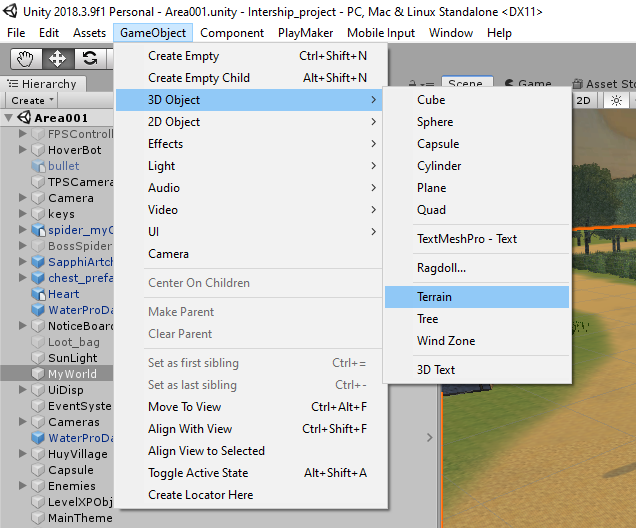
\includegraphics[width=1\linewidth]{intructions/1.png}
 		  		\captionof{figure}{Create terrain}
 		  		\label{fig:test2}
 		  	\end{minipage}
 		  	\begin{minipage}{.4\textwidth}
 		  		\centering
 		  		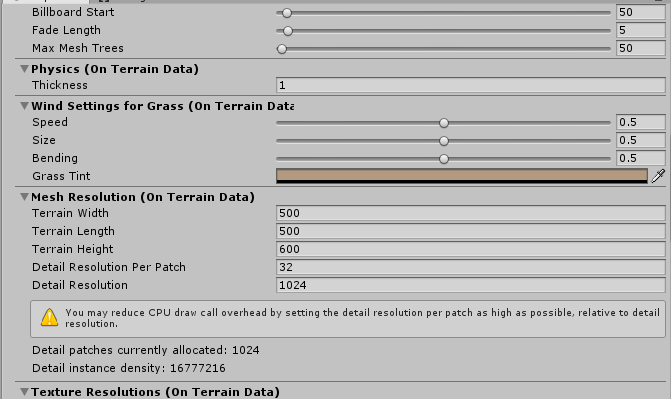
\includegraphics[width=1.4\linewidth]{intructions/2.png}
 		  		\captionof{figure}{Properties}
 		  		\label{fig:test3}
 		  	\end{minipage}
 		  \end{figure}
 	  \\[0.15cm]
 	  From the Inspector section, there are 3 sections: Paint texture, paint trees, paint details. Each of these sections has painting tool with 20 brush presets, resizable brush size, opacity. For the textures, we can use any texture we want for the terrain, as a case in point, I use this texture from this website: \href{https://www.textures.com/download/grass0153/48704}{https://www.textures.com/download/grass0153/48704}. The same applied for painting details, but for painting trees, the material for this one is 3D model, however it can be found in the Standard Assets which comes with Unity when installed. 
 	   \begin{figure}[h]
 	   	 \centering
 	   	 \begin{minipage}{1\textwidth}
 	   	 	\centering
 	   	 	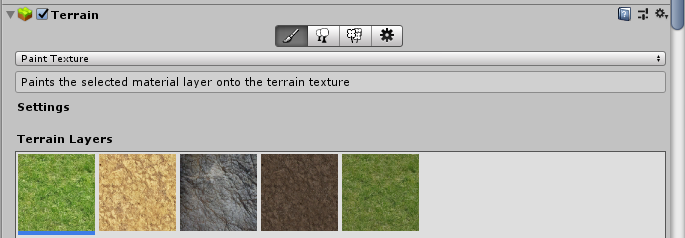
\includegraphics[width=0.75\linewidth]{intructions/3.png}
 	   	 	\captionof{figure}{Sections}
 	   	 	\label{fig:test4}
 	   	 \end{minipage}
 		 \end{figure}  
 		 
 	Besides, in order to make the terrain look better, the user can also raise or lower the terrain to create mountains, river. After finish creating the terrain, all we have to do is drag and drop other objects/prefabs into the scene, put the textures corresponding to each object, while these prefabs/objects can be found on Unity assets store or from free3d website as I mentioned from the introduction. 
 	 \paragraph{Player}
 	 To be able to interact with the objects, NPCs, a player should be added into the scene. For example, I use a little robot for my player. This model is free to download: \href{https://free3d.com/3d-model/bb8-35865.html}{https://free3d.com/3d-model/bb8-35865.html}.
 	 
 	 \begin{figure}[h]
 	 	\centering
 	 	\begin{minipage}{1\textwidth}
 	 		\centering
 	 		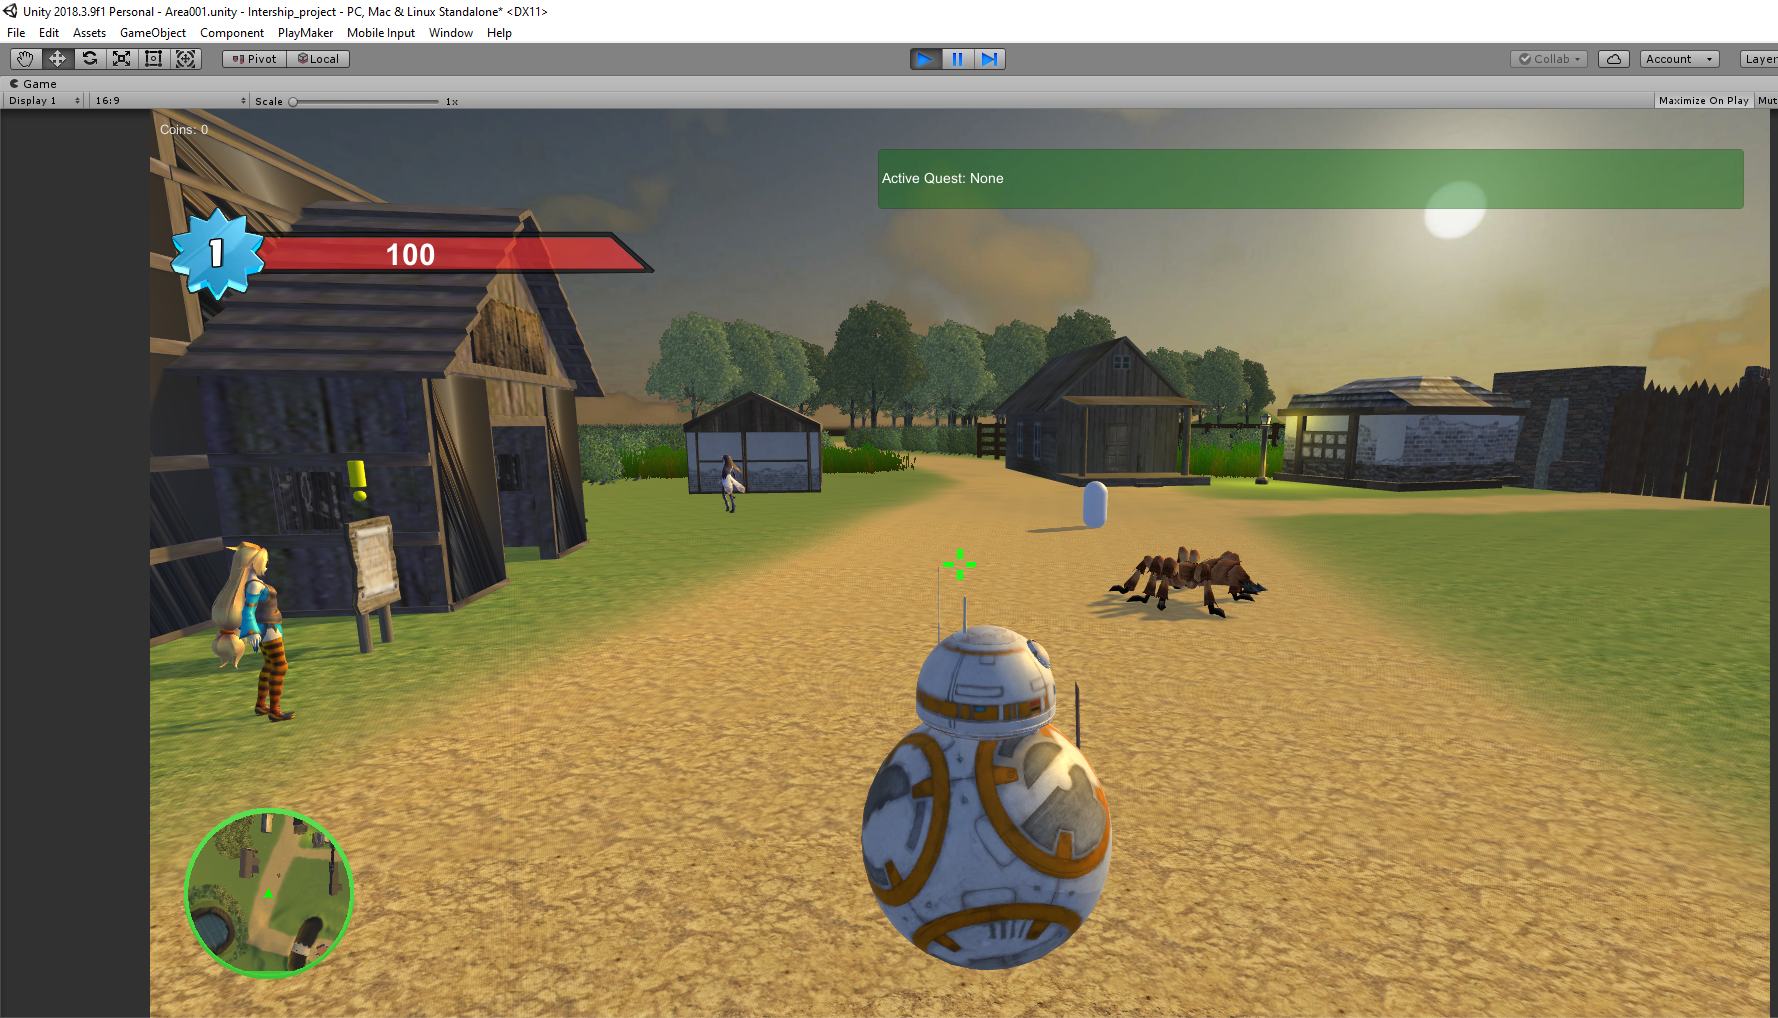
\includegraphics[width=0.75\linewidth]{intructions/4.png}
 	 		\captionof{figure}{Character example}
 	 		\label{fig:test5}
 	 	\end{minipage}
 	 \end{figure}
 	  
 	 Initially, the player will not move without any scripts attached to it, so I write a simple C\# script to control the player using visual studio and then attach the script to the player. Although there is a character controller prefab in the Unity's standard asset, which can be used, controlled instantly without doing anything. In this project, we'll not use character controller prefab, so that we can easily customize our character controller script later. \\[0.25cm] By default, when initializing a Unity project, there is already a camera called "Main camera", which is what the user can see from the game view in the hierarchy.  
 	 \\[0.25cm] From now, I am going to explain how can I implement character controller to move my character. Firstly, I have to find the input by go to Edit -> Project Settings -> Input. In the input section, Unity already implements 2 inputs named : "Horizontal" , "Vertical", along with Negative Button and Positive Button, and I can also add my own custom input in project setting. This is where I can move my character left and right, forward and backward. After finding the input, I can get the input by using: 
 	 \definecolor{codebackground}{rgb}{0.95, 0.95, 0.92}
 	 \lstdefinestyle{customc}{
 	 	belowcaptionskip=1\baselineskip,
 	 	breaklines=true,	
 	 	keepspaces       = true,
 	 	columns          = flexible,
 	 	backgroundcolor  = \color{codebackground},
 	 	xleftmargin=\parindent,
 	 	language=C,
 	 	showstringspaces=false,
 	 	basicstyle=\footnotesize\ttfamily,
 	 	keywordstyle=\bfseries\color{green!40!black},
 	 	commentstyle=\itshape\color{purple!40!black},
 	 	identifierstyle=\color{blue},
 	 	stringstyle=\color{orange},
 	 }
  
  \lstset{style=customc, basicstyle=\fontsize{7.5}{4}\ttfamily, language=C}
 	 \begin{lstlisting}
 	  Vector2 input = new Vector2(Input.GetAxis("Horizontal"), 
 	  Input.GetAxis("Vertical"));
 	 \end{lstlisting}
 	 Next, I have to normalize the input vector to see which direction the player has to move , face correctly. To be more specify, let's consider two trigonometry circles below:
 	
 	 		\definecolor{qqwuqq}{rgb}{0.,0.39215686274509803,0.}
 	 		\definecolor{ffqqqq}{rgb}{1.,0.,0.}
 	 		\definecolor{uuuuuu}{rgb}{0.26666666666666666,0.26666666666666666,0.26666666666666666}
 	 		\begin{tikzpicture}[line cap=round,line join=round,>=triangle 45,x=0.5cm,y=0.5cm]
 	 		\clip(-17.62,-11.46) rectangle (13.08,6.28);
 	 		\draw [shift={(-10.3,-3.27)},line width=0.5pt,color=qqwuqq,fill=qqwuqq,fill opacity=0.10000000149011612] (0,0) -- (0.4233601239113539:0.6) arc (0.4233601239113539:49.49045192111633:0.6) -- cycle;
 	 		\draw [line width=0.5pt] (-14.36,-3.3)-- (-6.24,-3.24);
 	 		\draw [line width=0.5pt] (-10.3,-3.27) circle (2.030055417962771cm);
 	 		\draw [line width=0.5pt] (-10.3,-3.27)-- (-6.24,-3.24);
 	 		\draw [line width=0.5pt] (-10.33,0.79)-- (-10.27,-7.33);
 	 		\draw [line width=2.8pt,color=ffqqqq] (-10.3,-3.27)-- (-7.662654488417639,-0.1831069580342808);
 	 		\draw [line width=0.5pt] (-7.662654488417639,-0.1831069580342808)-- (-7.639990169721227,-3.2503447549486797);
 	 		\draw (-10.74,1.68) node[anchor=north west] {90};
 	 		\draw [line width=0.5pt] (1.77,-3.3) circle (2.030055417962771cm);
 	 		\draw [line width=0.5pt] (-2.25,-3.31)-- (5.87,-3.25);
 	 		\draw (-5.82,-2.98) node[anchor=north west] {0};
 	 		\draw (-15.86,-3.14) node[anchor=north west] {180};
 	 		\draw (-10.94,-7.76) node[anchor=north west] {270};
 	 		\draw (1.46,1.66) node[anchor=north west] {0};
 	 		\draw (6.42,-2.92) node[anchor=north west] {90};
 	 		\draw (1.28,-7.96) node[anchor=north west] {180};
 	 		\draw (-3.74,-3.02) node[anchor=north west] {270};
 	 		\draw [line width=2.8pt,color=ffqqqq] (1.77,-3.3)-- (1.7404368698694395,0.7600032045968739);
 	 		\draw [line width=0.5pt] (1.77,-3.3)-- (1.7995631301305606,-7.3600032045968735);
 	 		\begin{scriptsize}
 	 		\draw [fill=uuuuuu] (-10.3,-3.27) circle (2.0pt);
 	 		\draw[color=black] (-8.94,-3.55) node {$X$};
 	 		\draw[color=black] (-7.32,-1.87) node {$Y$};
 	 		\draw[color=qqwuqq] (-9.22,-2.87) node {$\alpha$};
 	 		\draw [fill=uuuuuu] (1.77,-3.3) circle (2.0pt);
 	 		\end{scriptsize}
 	 		\end{tikzpicture}
 	 		{\\[-1.0cm]
 	 		\centering Figure 5.5: Two trigonometry circles}
 	 	\\[0.02cm]
 	 	From the left one above, suppose that the red line is the input direction, X and Y are vertical and horizontal components. Let's call the rotation angle of the character  {$\alpha$}. When looking at the two circles, it is clear that r is calculated as: 
 	 	\\[-0.5cm]
 	 	\[\alpha = arctan(\frac{Y}{X})\]
 	 	In Unity, however, if my character is looking forward, then it has the rotation of 0 (as seen from the right one), when facing right it has the rotation of 90 degree and so on. Let's call the rotation of character in Unity is r, when looking at the two circle, it's clearly that r is calculated as: \\[-0.5cm]
 	 	 \[r = 90 - \alpha; \hspace{0.8cm} or \hspace{1.0cm} r = arctan(\frac{X}{Y})\] 
 	 	By C\# code:
 	 	\begin{lstlisting}
 	 	float targetRotation = Mathf.Atan2(inputDir.x, inputDir.y) * Mathf.Rad2Deg;
 	 	transform.eulerAngles = Vector3.up * Mathf.SmoothDampAngle(transform.eulerAngles.y, targetRotation, ref turnSmoothVelocity, turnSmoothTime);
 	 	\end{lstlisting}
 	 	
 	 	Where Mathf.SmoothDampAngle is the function that can gradually change an angle given in degrees towards a desired angle by turnSmoothTime (in second). Vector3.up is used in the calculation so that the character will not rotate up or fly straight up.  \\[0.15cm] After that, to be able to move, transform.forward and Controller.Move is used here to move the character by a certain amount in the world space everytime when I press a button. \\[0.15cm] Finally, to finish setting up my character controller script, I have also added gravity, ability to jump for my character. From 10th grade, the equation to calculate the falling speed is defined as: 
 	 	\\[-0.5cm]
 	 	 \[v = \sqrt{2gh}\]
 	 	 where g is the gravity and h is the height the character begin to fall. As there is no air resistance in the game, this equation can be applied directly to the character following the script. For the ability to jump:
 	 	 \begin{lstlisting}
 	 	 if (controller.isGrounded)
 	 	 {
 	 	 	float jumpVelocity = Mathf.Sqrt(-2 * gravity * jumping);
 	 	 	VelocityY = jumpVelocity;
 	 	 }
 	 	 Vector3 velocity = transform.forward * currentSpeed + Vector3.up * VelocityY;
 	 	 controller.Move(velocity * Time.deltaTime);
 	 	 
 	 	 if (controller.isGrounded)
 	 	 {
 	 	 	VelocityY = 0;  
 	 	 }
 	 	 \end{lstlisting}
 	 	 Where VelocityY is defined as the falling speed equation above. As soon the character hit the ground, the character won't be able to fall anymore, so I have to assign VelocityY = 0 when controller.isGrounded. 
 	 \paragraph{Cameras}
 	 \begin{itemize}
 	 	\item \bfseries TPSCamera (Third Person Camera) 
 	 \end{itemize}
 	 
 	 Now we need to make a script to force the camera to follow the character. To do that, let's implement transform.position = Target.position - transform.forward * distFromTarget , where the Target variable is the character object. The reason I put minus transform.forward * distFromTarget is to make sure that the camera always behind the character, not in front of him. 
 	 \begin{figure}[h]
 	 	\centering
 	 	\begin{minipage}{.4\textwidth}
 	 		\centering
 	 		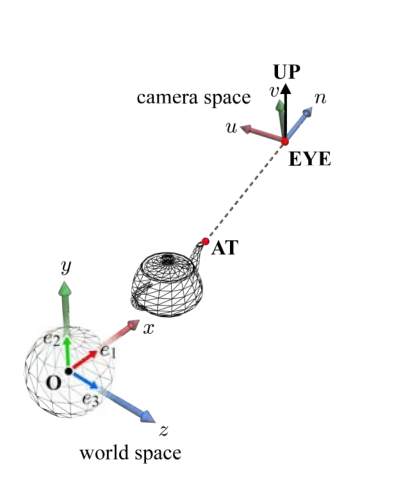
\includegraphics[width=0.7\linewidth]{intructions/camera_space.png}
 	 			\centering
 	 		\captionof{figure}{Camera world space \\[0.01cm] (Image from number \cite{3D} in reference section)}
  			\label{fig:test7}
  		\end{minipage}
 	 \end{figure}  
  	\\[0.05cm]
 	 The camera is specified in term of three parameters: {\bfseries EYE, AT}, and {\bfseries UP}, as show in the left one. EYE is the camera position, AT is the reference point the camera is pointing at, and UP usually is set to the y-axis of the world space. For example, in the right one, AT is set at the position a little bit above the character for not covering the center of the screen which I am going to explain why later.
 	 After that, the camera needed to be rotated around with a mouse because I'd like to see what is happening around the character. And the same applied to the character controller script, but this time, I use Input.GetAxisRaw function instead of GetAxis is because I don't want the rotating to be smooth immiately as it can cause a short delay as GetAxisRaw will only return 0,-1 or 1 while GetAxis change gradually from 0 to 1 or 0 to -1.  
 	 Moreover, the function Lerp is used here instead of SmoothDamp due to the fact that the smoothdamp function adds the curve which can cause delay, for instance, when I stop moving my mouse, the camera still moving, while Lerp only behaves linear. As now, there is still one more problem, on the mouseY rotation, the camera can be rotated 360 degree which is not I wanted, so I used the function Mathf.Clamp to limit the rotation of the mouseY axis, the minimum, maximum here is -40, 85 degree for the third person camera controller. In the end, to finish my TPS camera controller, I've modified the character controller script a bit by adding cameraT.eulerAngles.y in the targetRotation where cameraT is the MainCamera(the TPS camera), to make sure that the camera will following the player correctly.
 	 
 	  \begin{itemize}
	 	\item \bfseries Camera Collision and Occlusion Detection  	 	
 	 \end{itemize}
 	 In some situations, like in the figure below, when the camera collide with the wall or the wall comes in between the character and the camera, they're called occlusion and collision. When the camera goes through the wall or the ground, it can cause shearing.
 	 \begin{figure}[h]
 	 	\centering
 	 	\begin{minipage}{.4\textwidth}
 	 		\centering
 	 		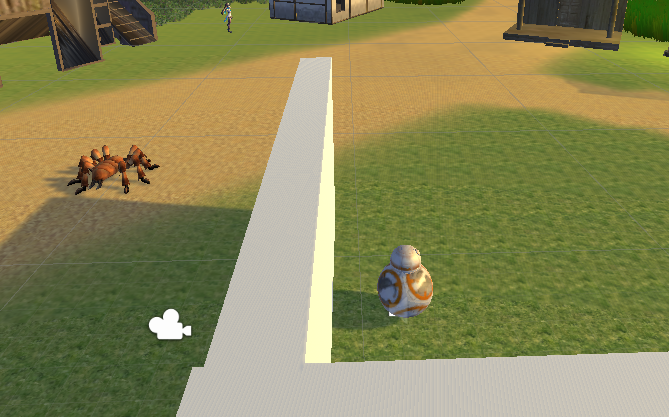
\includegraphics[width=1\linewidth]{intructions/camera_cover.png}
 	 		\centering
 	 		\captionof{figure}{Occlusion example}
 	 		\label{fig:test8}
 	 	\end{minipage}
  	\begin{minipage}{.4\textwidth}
  		\centering
  		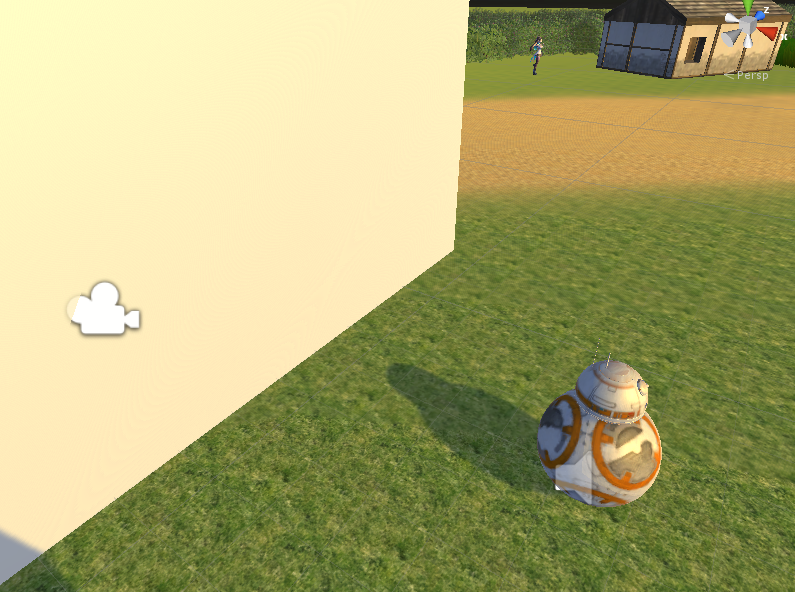
\includegraphics[width=1\linewidth]{intructions/camera_collide.png}
  		\centering
  		\captionof{figure}{Collision example}
  		\label{fig:test9}
  	\end{minipage}
 	 \end{figure}
  \\[0.15cm]
  So, the goal here is to handle {\bfseries Collision} and {\bfseries Occlusion} with as little shearing as possible. Let's defined each one of these underlined terms really means. 
  \begin{figure}[h]
  	\centering
  	\begin{minipage}{.4\textwidth}
  		\centering
  		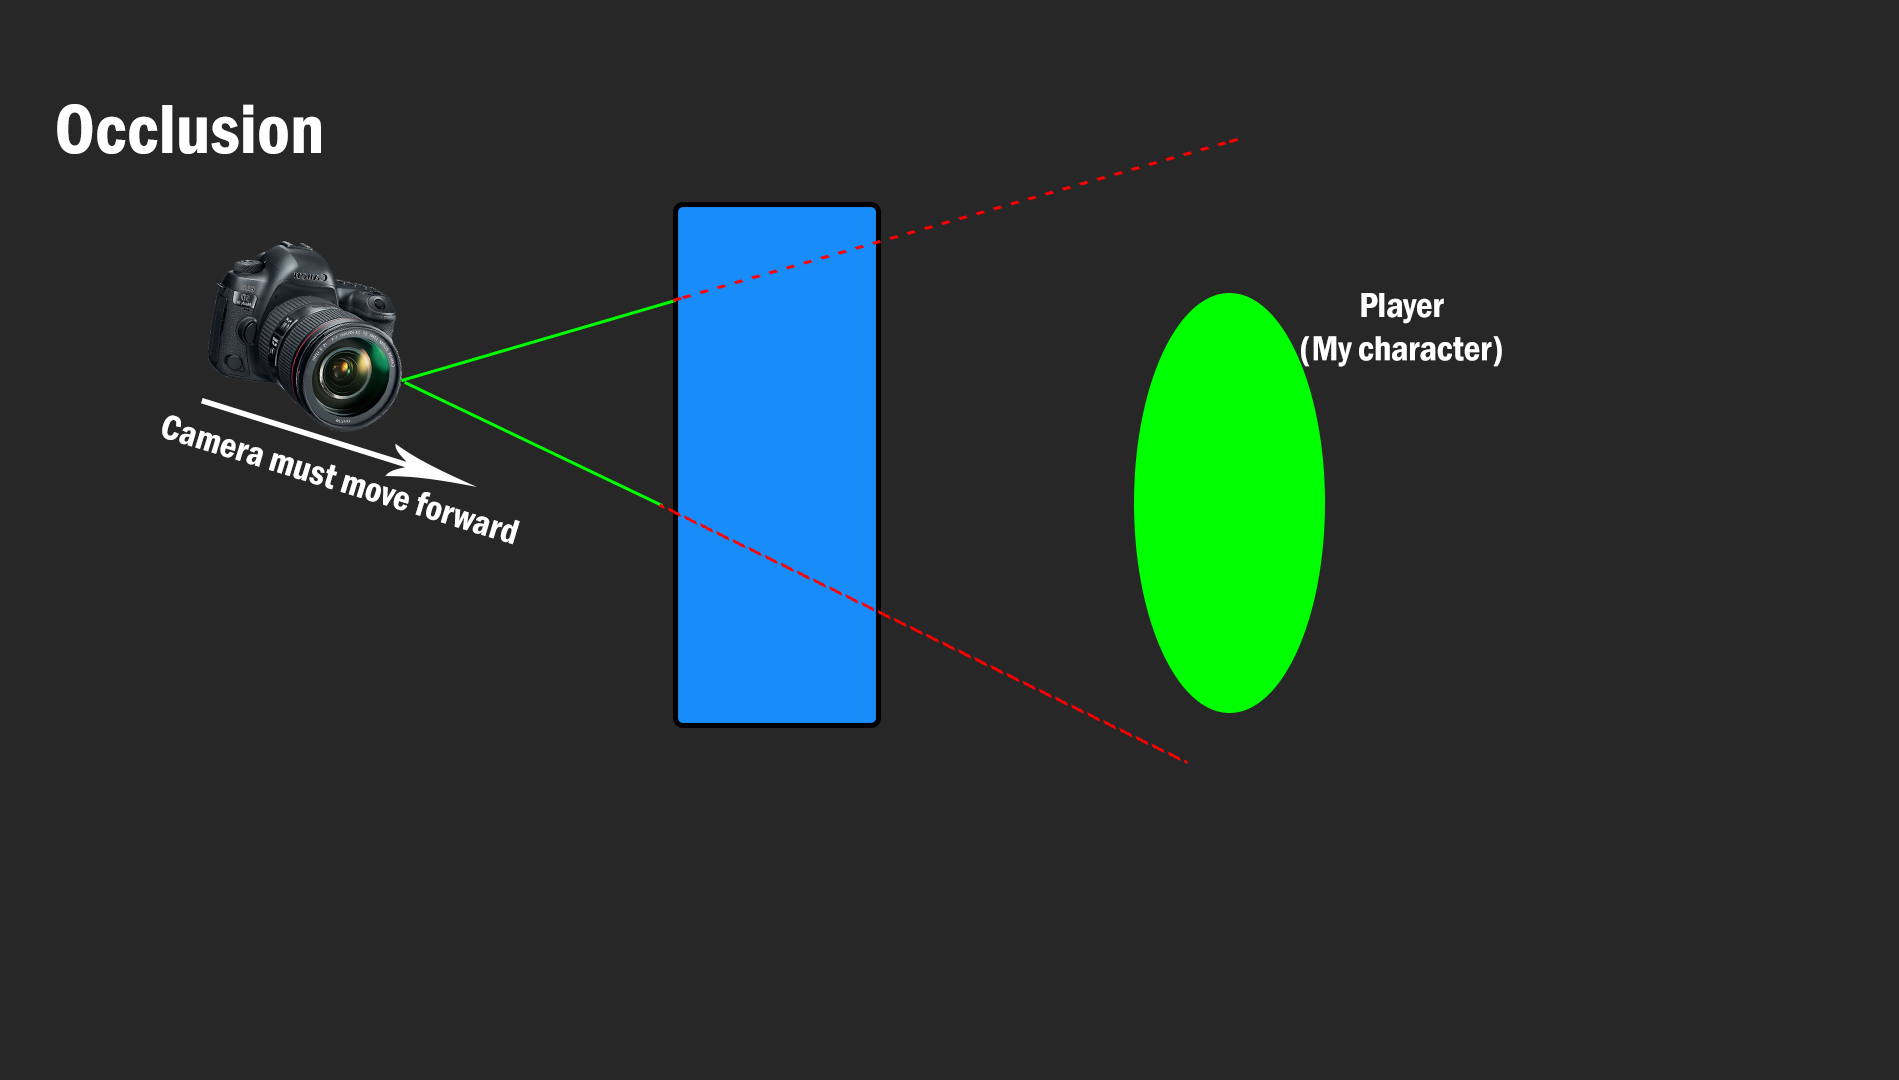
\includegraphics[width=1.3\linewidth]{intructions/Occlusion_camera.png}
  		\centering
  		\captionof{figure}{Occlusion}
  		\label{fig:test10}
  	\end{minipage}
  \end{figure}
  \\[0.15cm]
  Occlusion is when the game is running where the pillar or the wall comes in between the character and the camera view, the character is no where to be seen, and I need to move forward if that happen. Like the figure above, if the camera is not hitting anything but its view is being obstructed, I will have to move it forward so that the camera can see the player.
  \begin{figure}[h]
  	\centering
  	\begin{minipage}{.4\textwidth}
  		\centering
  		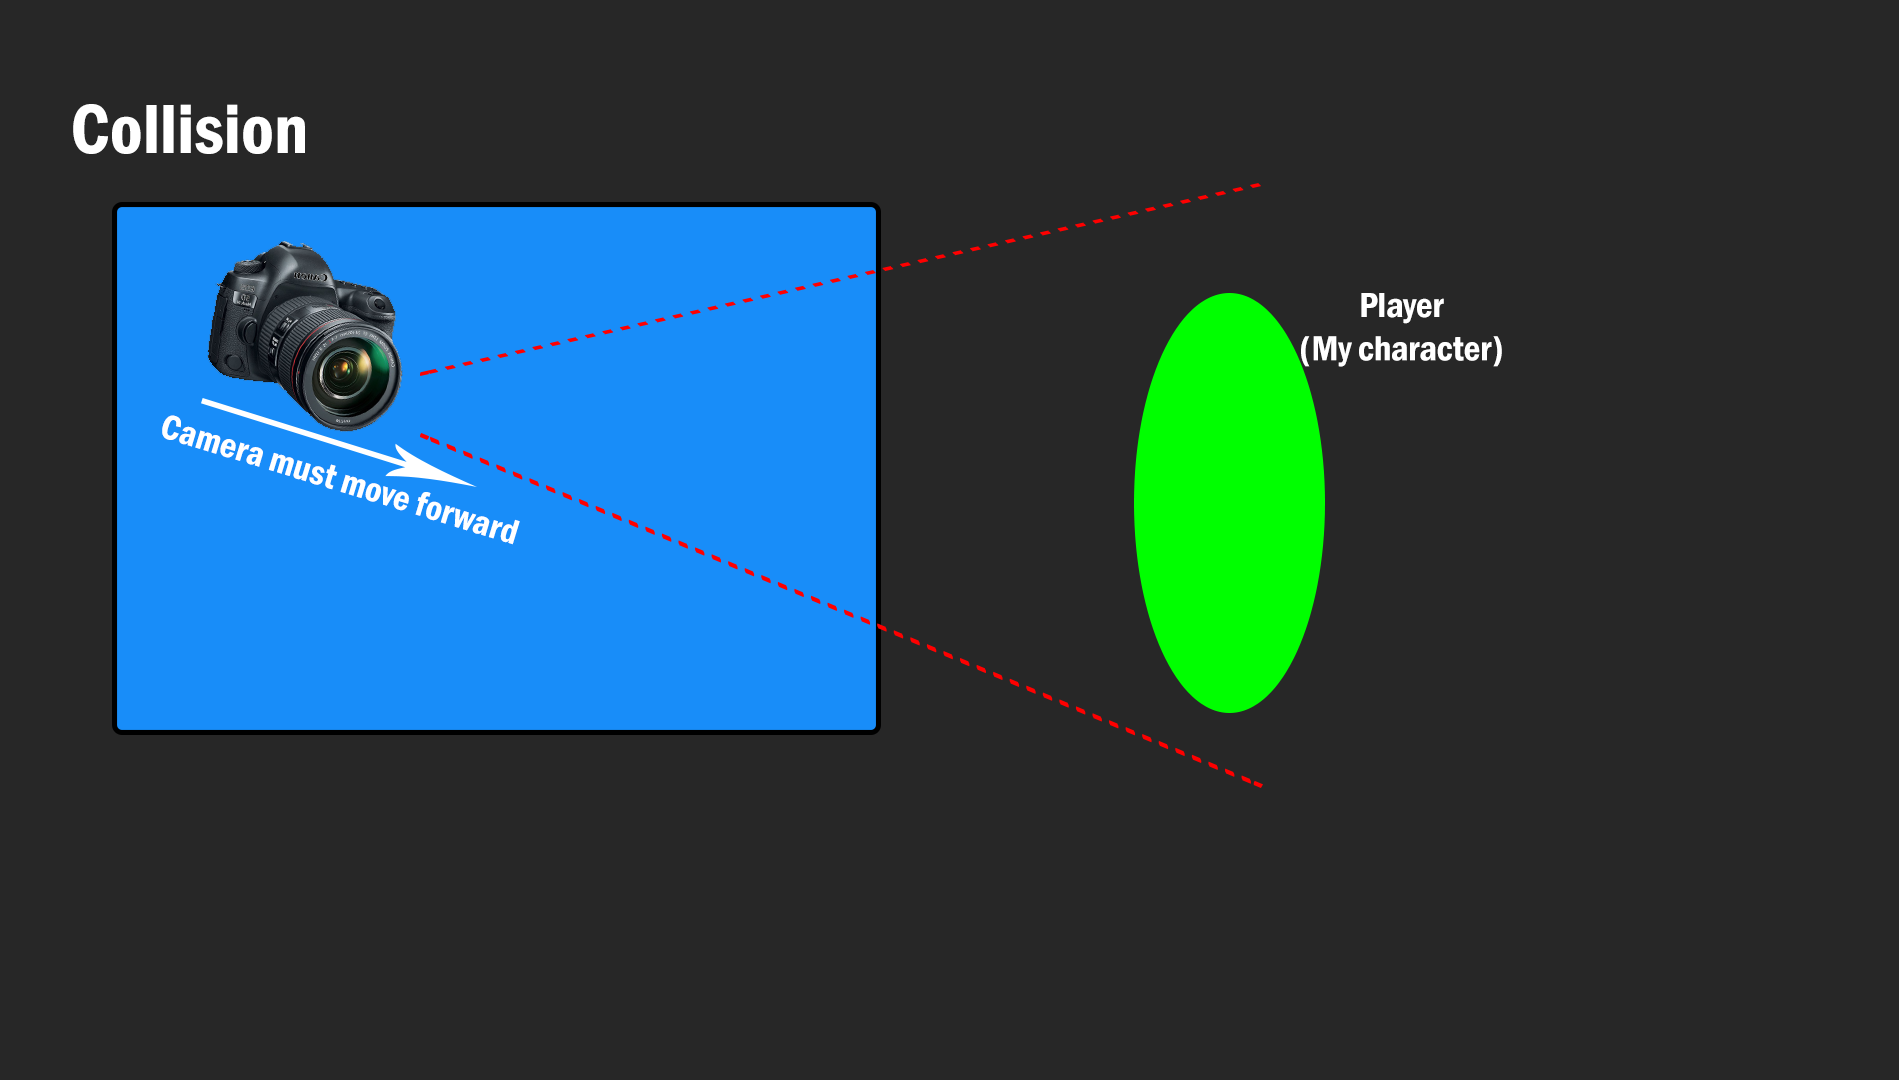
\includegraphics[width=1.3\linewidth]{intructions/Collision_camera.png}
  		\centering
  		\captionof{figure}{Collision}
  		\label{fig:test11}
  	\end{minipage}
  \end{figure}
 \\[0.05cm]
  Collision is where the camera actually does hit something and the view is still obstructed so I still need to move the camera forward. 
  \\[0.05cm] From these, it's actually a problem that can be solved with one solution. I am going to determine if the camera can see the player in a moment , if a point of the camera cannot see the player then the camera should be moved forward, whenever it's collision or occlusion, it's still the same issue. And shearing is when the camera go through the wall, I am able to see through the wall too, to where I see the open space, even the skybox. It's really detract from the realism of the scene,so I have to limit the shearing as much as possible.  	
  \\[0.15cm]
  Before solving the problem, let's implement some definition of the Camera.
  \newpage
  \begin{figure}[h]
  	\centering
  	\begin{minipage}{.4\textwidth}
  		\centering
  		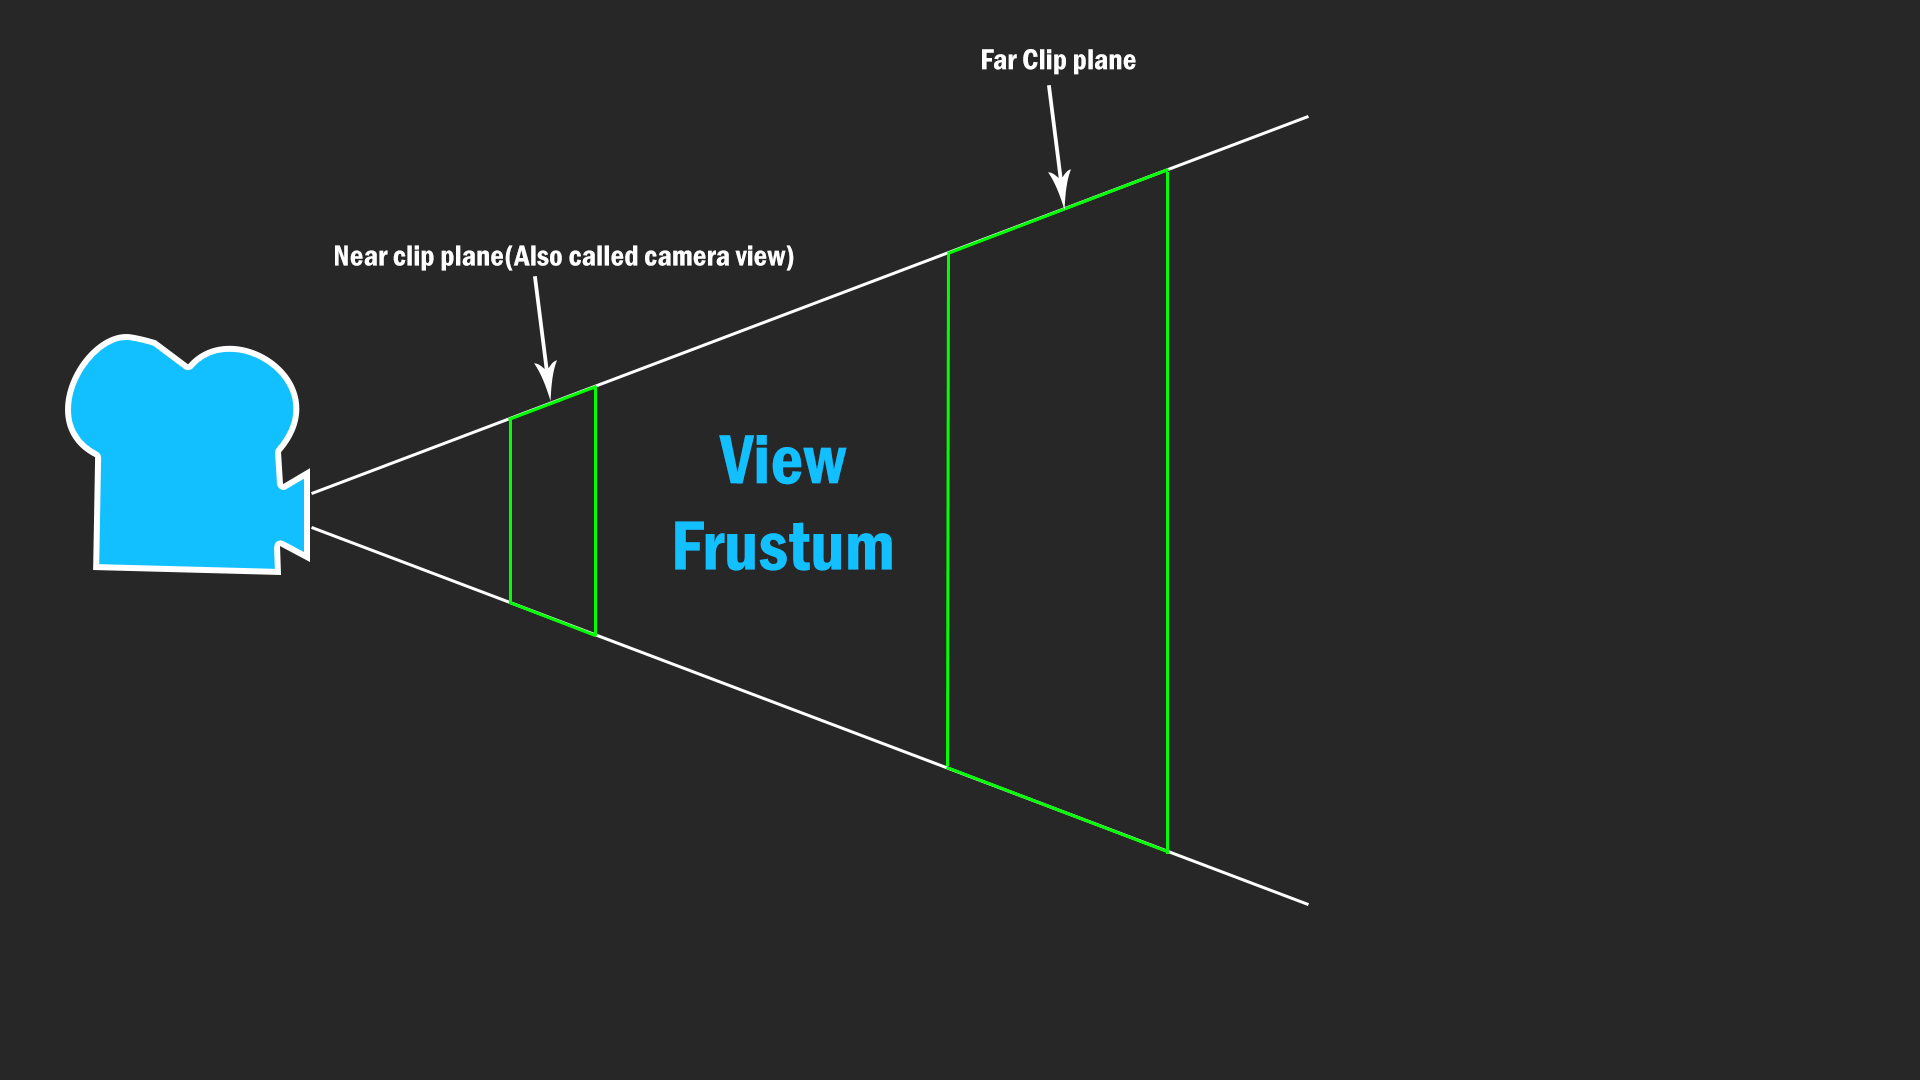
\includegraphics[width=1.7\linewidth]{intructions/Camera_overview.png}
  		\centering
  		\captionof{figure}{Camera overview}
  		\label{fig:test12}
  	\end{minipage}
  \end{figure} 
From the image above, 2 white lines are defines as a view angle. Inside the view angle, there is also a clip plane defined by the green rectangle, which is also the camera view. And at the center of the near clip plane is where the camera is pointing at, and at that point, I've drawn the crosshair, to make sure that this is the camera position. This is the position where the character can interact with the objects, NPCs so as I mention above in the character section, that's why the character cannot be at the middle of the near clip point. The second green rectangle is defined as the far clip plane, which determines how far out into the world the camera view can see. And between the two plane is view frustum, within this shape is what I can see in the game preview.
\\[0.05cm] To detect if the camera cannot see the player or the camera is collided with the objects, all I have to do is just a simple raycasting from the character to the camera, and what is raycasting, I'll explain in the next section. 
\begin{figure}[h]
	\centering
	\begin{minipage}{.4\textwidth}
		\centering
		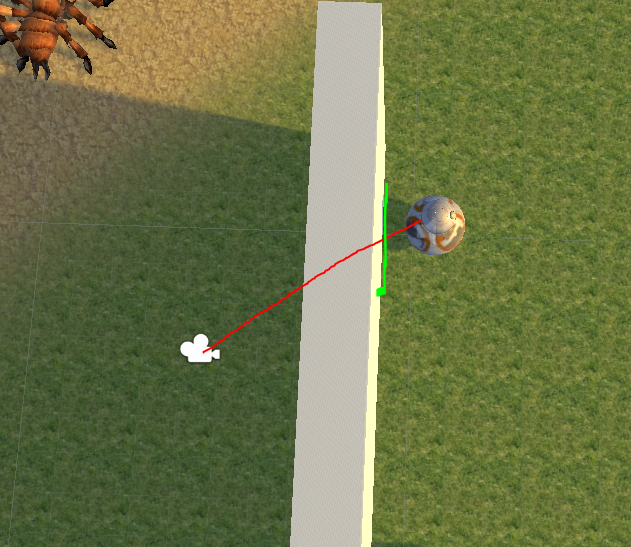
\includegraphics[width=1.3\linewidth]{intructions/raycasting.png}
		\centering
		\captionof{figure}{Occlusion}
		\label{fig:test13}
	\end{minipage}
\end{figure} 
\\[0.05cm]
The best raycasting function to use here is Physics.LineCast, as it can return true if the camera hit something, vice versa. This function works in both Collision and Occlusion situation. Like the image above, I've drawn the LineCast between the character and the camera using the function Physics.LineCast, whenever the camera is behind the wall and the player or being collided with the wall, the line can still hit the objects, return true. 
\begin{lstlisting}
void CollisionCheck(Vector3 ReturnPoint)
{
	RaycastHit hit;
	if (Physics.Linecast(Target.position, ReturnPoint, out hit, collisionMask))
	{
		normal = hit.normal*wallPush;
		p = hit.point + normal;
		if (Vector3.Distance(Vector3.Lerp(transform.position, p, moveSpeed * Time.deltaTime), Target.position) <= EvenCloserDistance)
		{

		}
		else
		{
			transform.position = Vector3.Lerp(transform.position, p, moveSpeed * Time.deltaTime);
		}
		return;

	}
	transform.position = Vector3.Lerp(transform.position, ReturnPoint, returnSpeed * Time.deltaTime);
}
\end{lstlisting}
From the code above, the hit function is to return the information where the line hit, collisionMask determine which object layer should the line hit. After the line hit something, I've defined the function hit.normal to find the normal if the line hit the wall, and if it hit, the value will be 1, and the vector p is the position the camera should move. The reason why I do the normalize, add it with the hit.point is just to prevent the camera from clipping with the object when the camera start to move. Finally, to make sure that when occlusion happen, the camera still move to the correct position, be able to see the player, I measure the distance between the camera point and the player, if it's already smaller than a specific value than stop moving the camera, otherwise, it'll lerp to the correct position in order to see the player.  
\begin{itemize}
	\item \bfseries FPSCamera 	 	
\end{itemize}
	This camera represents how we see the world in reality, everyday life. The controller script for this one is basically the same as the TPScamera script I've written before, but the only difference is the FoV, it's a bit narrower than the FoV of TPScamera and the clamp angle. The camera position is right at the position of the eye's character, for making the gameplay looks more realistic. Moreover, I've written the script to allow the user to change between the FPS mode and TPS mode by pressing V. One more thing, to be able to synchronized 2 camera, all I do is copy almost all the code lines from TPSCamera script and then paste to the FPS one, so that 2 camera will rotate , move extractly at the same angle, same speed. 

\paragraph{RayCasting}
  A Raycast is conceptually like a beam that's fired from a point in space along a particular direction. Any object making contact with the beam can be detected and reported. With the ability to get information from the object that the beam hit, this is the main method for this project, as the character is able to interact with other objects in the virtual world. In Unity, raycast support both 2 dimension and 3 dimension, and for my project, I'll use 3d version for working with 3D space. there are two type of raycast that's usually used, Physics.Raycast and Physics.Linecast.
  \begin{itemize}
  	\item \bfseries Physics.Raycast(Vector3 origin,  Vector3 direction, float maxDistance = Mathf.Infinity, out hit, layerMask)	 	
  \end{itemize}
 	This type of function casts a ray from the original point, which is Vector3 origin into direction point (Vector3 direction) with the length of maxDistance. Normally, the maxDistance usually set to Mathf.Infinity for casting to the infinite length. This function will return true if the ray intersects with something, otherwise false. The fourth variable, the out usually passed by hit, it provides the info about what it hit, like the distance from the origin to the point or the position where it hit, which is extractly what I need for my character to be able to interact, communicate with other objects in the scene.
 	\begin{figure}[h]
 		
 		\begin{minipage}{1\textwidth}
 			\centering
 			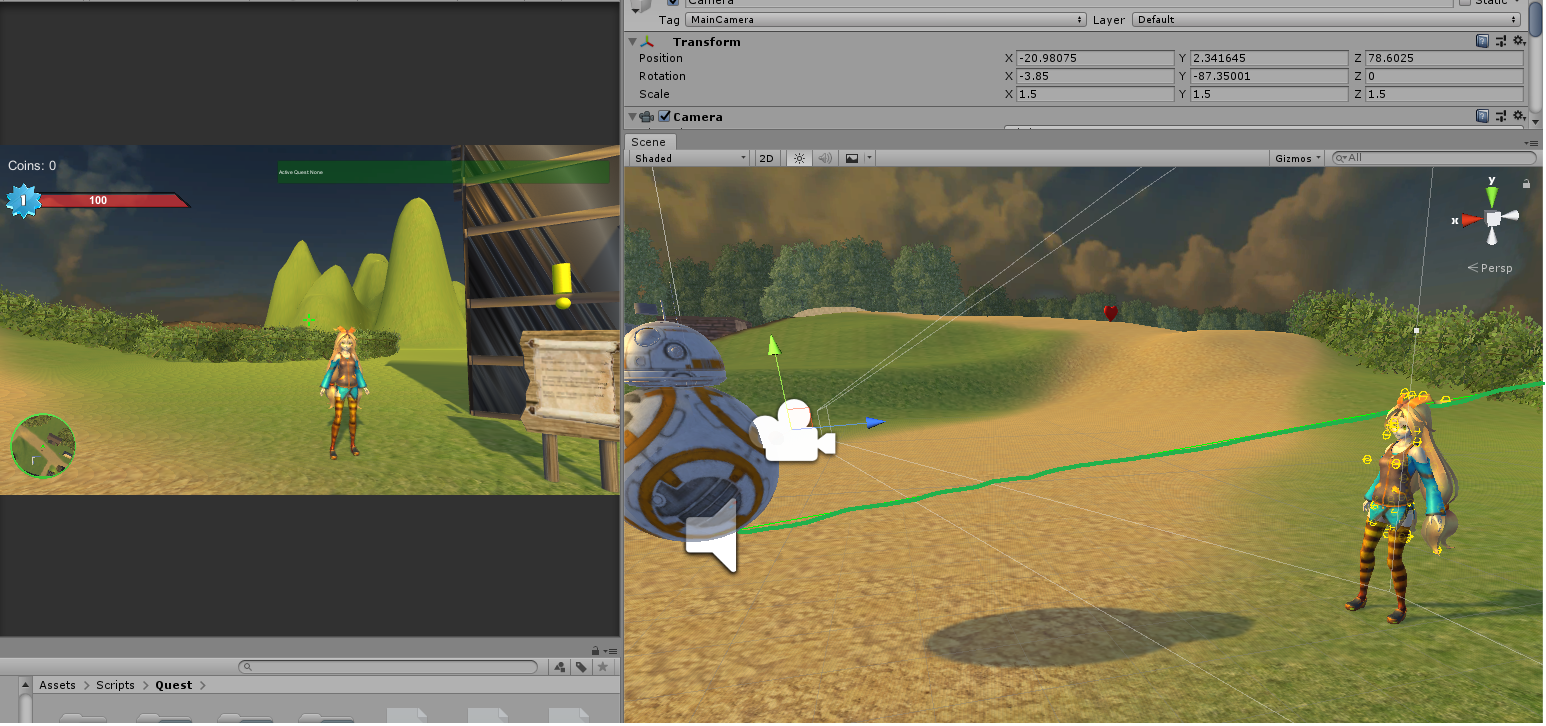
\includegraphics[width=1\linewidth]{intructions/RayCast_example1.png}
 			\centering
 			\captionof{figure}{RayCast example}
 			\label{fig:test14}
 		\end{minipage}
 	
 	\end{figure} 
 	
 	For example, from the figure 13, the greens line is actually the ray drawn from raycast. In the scene above, this ray will provide the distance between my character and the object it hit by hit.distance. In this situation, as the player is far from this NPC, the text which I have defined before will not pop to the screen, but when I move close to the NPC, the text actually pops up: "[E] talk to NPC"
 	\begin{figure}[h]
 		
 			\begin{minipage}{1\textwidth}
 				\centering
 				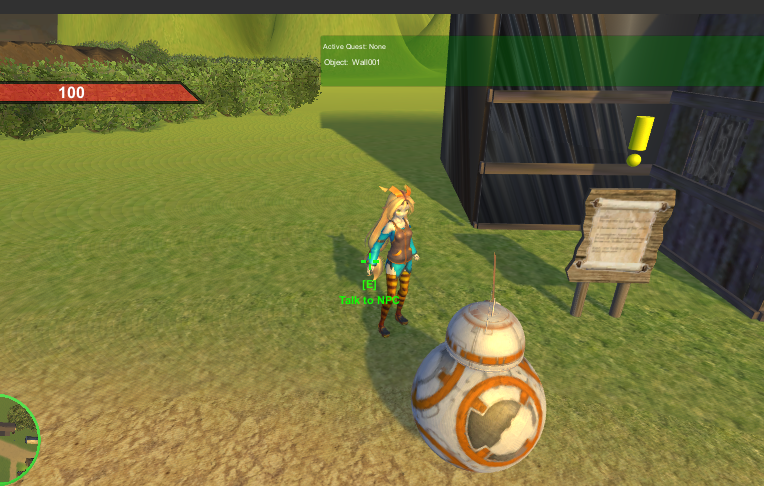
\includegraphics[width=0.5\linewidth]{intructions/text_popup.png}
 				\centering
 				\captionof{figure}{Text popup}
 				\label{fig:test15}
 			\end{minipage}
 		\end{figure}
 	\\[0.05cm]
 	This is because I've declared a float variable, when hit.distance bigger than that variable, the text will not appear until hit.distance is smaller. This is the concept of communicating with objects in the scene. Besides, the out variable can be used to get the object name where the ray hit by using hit.collider.gameObject.name: 	
 	\noindent\begin{minipage}{0.3\textwidth}
 		
\includegraphics[width=\linewidth]{intructions/objectname.png}
 	\end{minipage}
 	\begin{itemize}
 		\item \bfseries Physics.Linecast(Vector3 start,  Vector3 end , out hit, , layerMask)	 	
 	\end{itemize}
 		This function is pretty similar to the raycast function, although they both return true if the ray intersect with a collider, only recognize objects that have collider. The only difference between these two raycasting method is that the raycast only trigger the collider that starts outside of the origin object, and then intersects,  while the linecast is not, it will still trigger the collider of the beginning point. That's why I didn't use physics.raycast method for my camera collision detector, as physics.linecast trigger both the collider of two points.
 
	\paragraph{Bump mapping}
	In order to make the object surface look more realistic, bump mapping is a technique in computer graphic to do that by simulating small displacements of the surface. However, the number of polygons does not increase. The modified surface heavily relied on light reflection, define how the light should shine on the surface.
	The method to perform bump mapping I am going to use here will be divided into 3 stages: height map, normal map and occlusion map, the most important one in this method are height map and normal map. In this project, since I'll only generate bump map from a simple 2D texture, I'll not go too deep into this method, make it as simple as possible. This's the way how Unity can perform bump mapping on the object surface.
	\begin{itemize}
		\item \bfseries Height map	 	
	\end{itemize}
		To be able to generate normal map, I'll need to create height map from the 2d texture first, to simulate the high of vertex, from that, I can simulate the dept, how the light can shine into the surface. A height map is used to fake depth or essentially height on areas of texture map, the larger the difference between the height and the black, the more the distance it will appear on the surface. For creating the height map, I'll use Photoshop to make it. The texture for generating  the height map is this brick texture, for example: 
		 \begin{figure}[h]
		 	\centering
		 	\begin{minipage}{.3\textwidth}
		 		\centering
		 		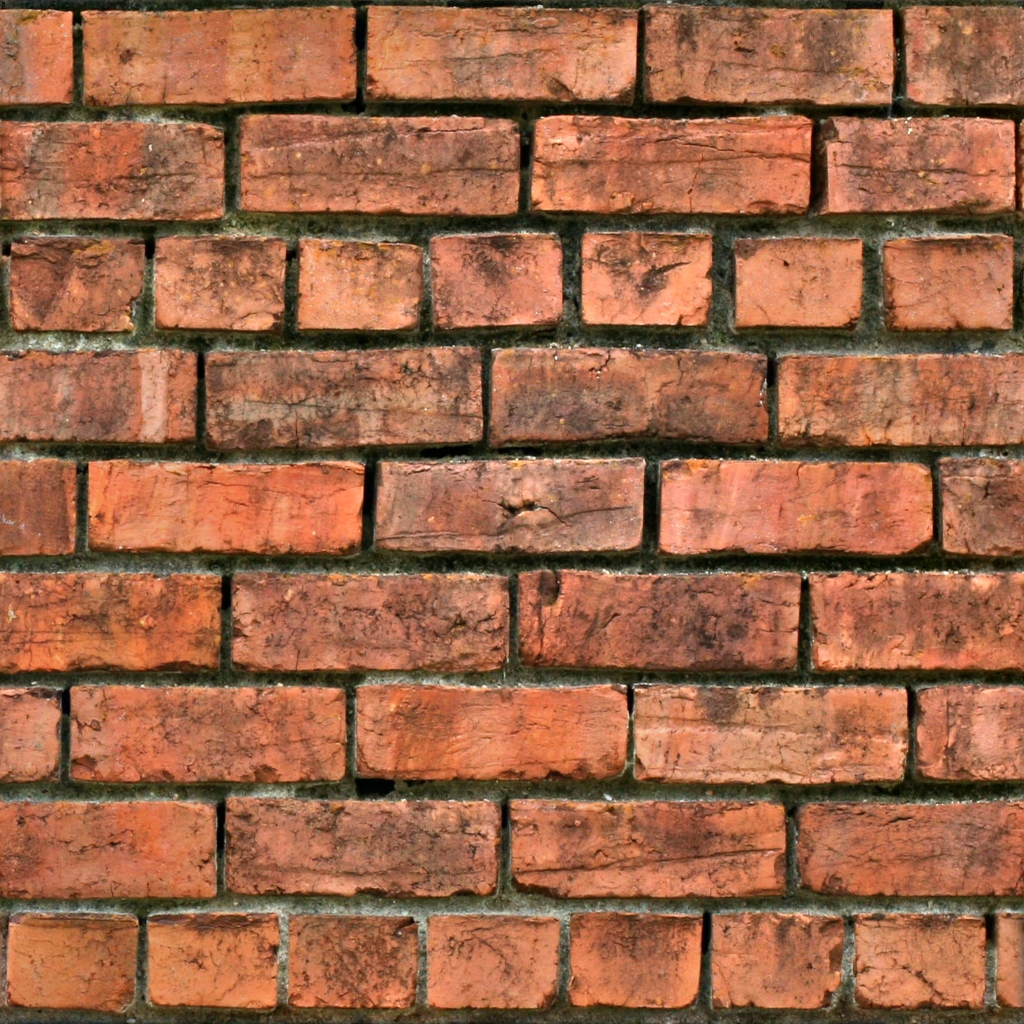
\includegraphics[width=0.8\linewidth]{intructions/Brick001.jpg}
		 		\centering
		 		\captionof{figure}{Original texture}
		 		\label{fig:test16}
		 	\end{minipage}
	 		\begin{minipage}{.25\textwidth}
	 			\centering
	 			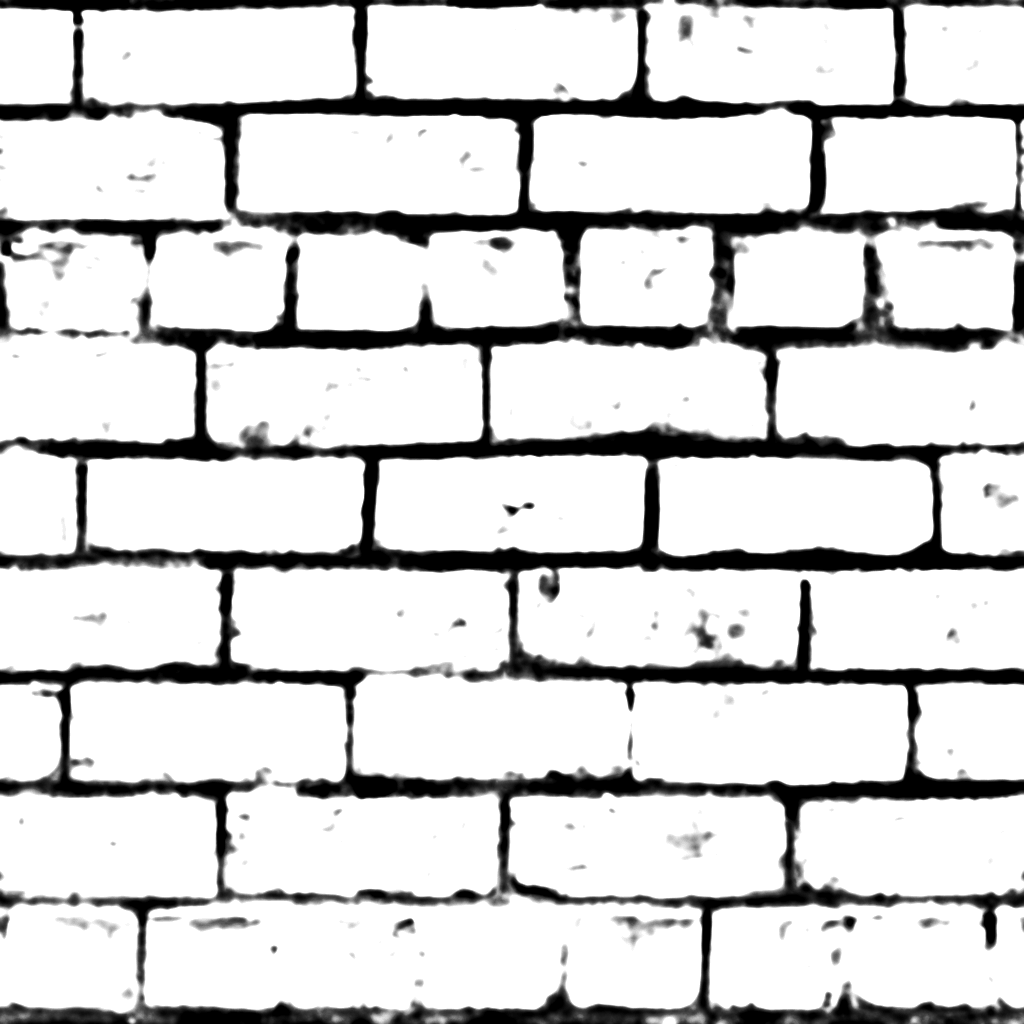
\includegraphics[width=0.8\linewidth]{intructions/Brick001_height.png}
	 			\centering
	 			\captionof{figure}{Height map}
	 			\label{fig:test17}
	 		\end{minipage}
 		\begin{minipage}{.25\textwidth}
 			\centering
 			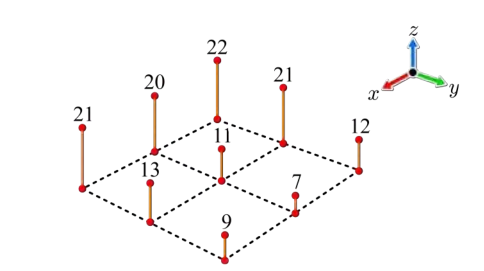
\includegraphics[width=1.4\linewidth]{intructions/height_example.png}
 			\centering
 			\captionof{figure}{Height map values \\[0.01cm] (Image from number \cite{3D} in reference section)}
 		\end{minipage}
 	\end{figure} 
 \\[0.02cm]
 Basically, the height image is the grey scale image with black and white range, so I'll convert the image to greyscale in Photoshop by selecting Image -> Adjustment -> Black and white. After creating the greyscale image, I'll try to modify the contrast by selecting a small circle at the bottom left, and choose level to adjust the black, white range, adjust the white area to become whiter, dark area to become even darker.
 \\[0.01cm]
 \noindent \begin{minipage}{0.21\textwidth}
 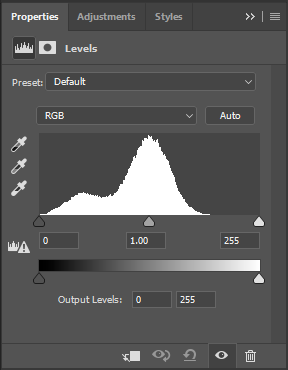
\includegraphics[width=\linewidth]{intructions/contrastAdjusting.png}
 \end{minipage}
  \\[0.2cm]
  If the height is in the range of [0,255], the lowest height 0 is colored in black, and the highest 255 is colored in white. As of now, there are still noises in the height map, I'll filter the noise by going to Filter -> Blur -> Gaussian Blur: \begin{minipage}{0.21\textwidth}
  	
\includegraphics[width=\linewidth]{intructions/guassian_blur.png}
  \end{minipage}  Depends on each textures, but for this one, 3.5 pixels is enough to filter the noises, for not losing the detail like in the figure 16, so that I'll get better result when creating the normal map.  
\begin{itemize}
	\item \bfseries Normal map	 	
\end{itemize}
  A normal map is a special kind of texture that allow us to add surface detail such as bumps, grooves, and scratches to a model which catch the light as if they are represented by real geometry, it contains surface normals. 
  \begin{figure}[h]
  	\begin{minipage}{.45\textwidth}
  		\centering
  		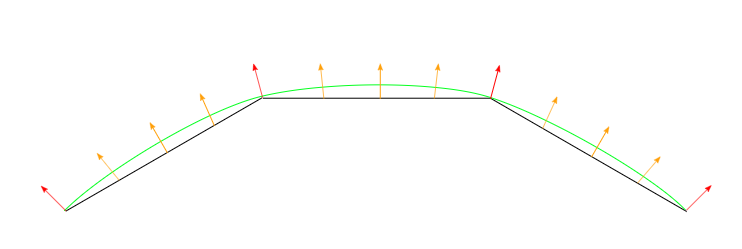
\includegraphics[width=1\linewidth]{intructions/surface_normal.png}
  		\centering
  		\captionof{figure}{Surface normal, across 3 polygons \\ Image from number \cite{Unity} in reference section}
  		\label{fig:test18}
  	\end{minipage}
  	\begin{minipage}{.4\textwidth}
  		\centering
  		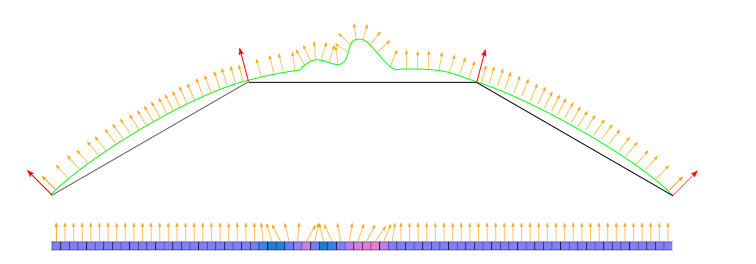
\includegraphics[width=1.6\linewidth]{intructions/surface_normal_across.png}
  		\centering
  		\captionof{figure}{Normal mapping across three polygons \\ (Image from number \cite{Unity} in reference section)}
  		\label{fig:test179}
  	\end{minipage}
  \end{figure}
 \\[0.01cm]
 The simplest way is to compute the surface normal from the height map as I created above at the point  (x,y,h(x,y)). Here, h represents the discrete height function, and x,y represent as the pixel coordinate. 
 \begin{figure}[h]
 	\begin{minipage}{1\textwidth}
 		\centering
 		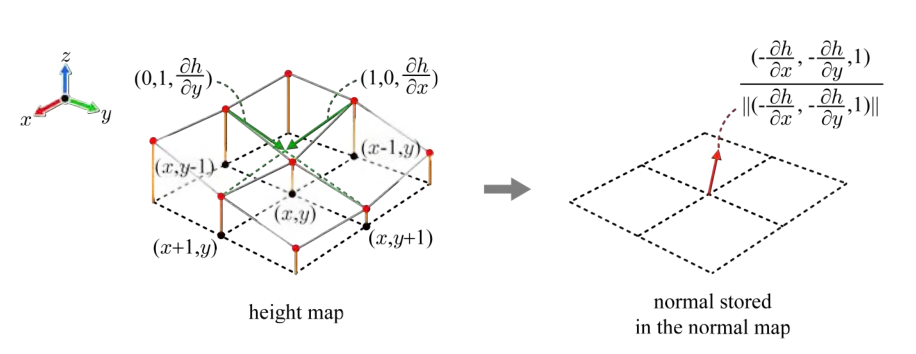
\includegraphics[width=0.7\linewidth]{intructions/normal_map_calculation.png}
 		\captionof{figure}{(Image from number \cite{3D} in reference section)}
 		\label{fig:test180}
 		\centering
 	\end{minipage}
 \end{figure} 
\newpage
In here, the partial derivatives are need for computing the normal: $\frac{\partial h}{\partial x}$ and $\frac{\partial h}{\partial y}$. They are defined by the height store at four neighbors of the pixel coordinate: \{(x + 1,y),(x $- 1$,y),(x,y + 1),(x,y $- 1$)\}. \\[0.01cm]The equation of these partial derivatives are: \begin{minipage}{1\textwidth}
	\scalebox{1.3} {$\frac{\partial h}{\partial x} = \dfrac{h(x + 1,y) - h(x - 1,y)}{2}$ }
	\\[0.04cm]
	\scalebox{1.3} {$\frac{\partial h}{\partial y} = \dfrac{h(x,y + 1) - h(x,y - 1)}{2}$ }
\end{minipage}
\\[0.2cm] After calculating these derivatives, the cross product is ({$-\frac{\partial h}{\partial x}$, $-\frac{\partial h}{\partial y}$, $1$), which is normalized and stored at (x,y). In the C\# function, this can be implemented as: \begin{lstlisting}
	private Texture2D GenerateNormal(Texture2D source)
	{
		normalTexture = new Texture2D(source.width, source.height, TextureFormat.ARGB32, true);
		for (int y = 0; y < normalTexture.height; y++)
		{
			for (int x = 0; x < normalTexture.width; x++)
			{
				xHeight = (GetColor((source.GetPixel(x+1, y) - source.GetPixel(x - 1, y)))-1)*0.5f;
				yHeight = (GetColor((source.GetPixel(x, y + 1) - source.GetPixel(x, y - 1)))-1)*0.5f;
				normalTexture.SetPixel(x, y, new Color(-xHeight, -yHeight, 1.0f, 1.0f));
	
			}
		}
		normalTexture.Apply();
		System.IO.File.WriteAllBytes("Assets/Sample001_n.png", normalTexture.EncodeToPNG());
		return normalTexture;
	}
	\end{lstlisting}
 Where x is the width and y is the height of image. The reason I minus the derivative functions with 1 is because I am trying to get the color value in the height map , and the normal value is calculated by this equation: $ Normal = (2.Color) - 1 $ so $ Color = \frac{Normal + 1}{2}$. And the SetPixel function is set by the negative derivative, so I should minus the normal with 1 instead of plus. With the normal map, the surface will look like in the picture below, as how the light shines on the surface.
 
 \begin{figure}[h]
 	\centering
 	\begin{minipage}{.3\textwidth}
 		\centering
 		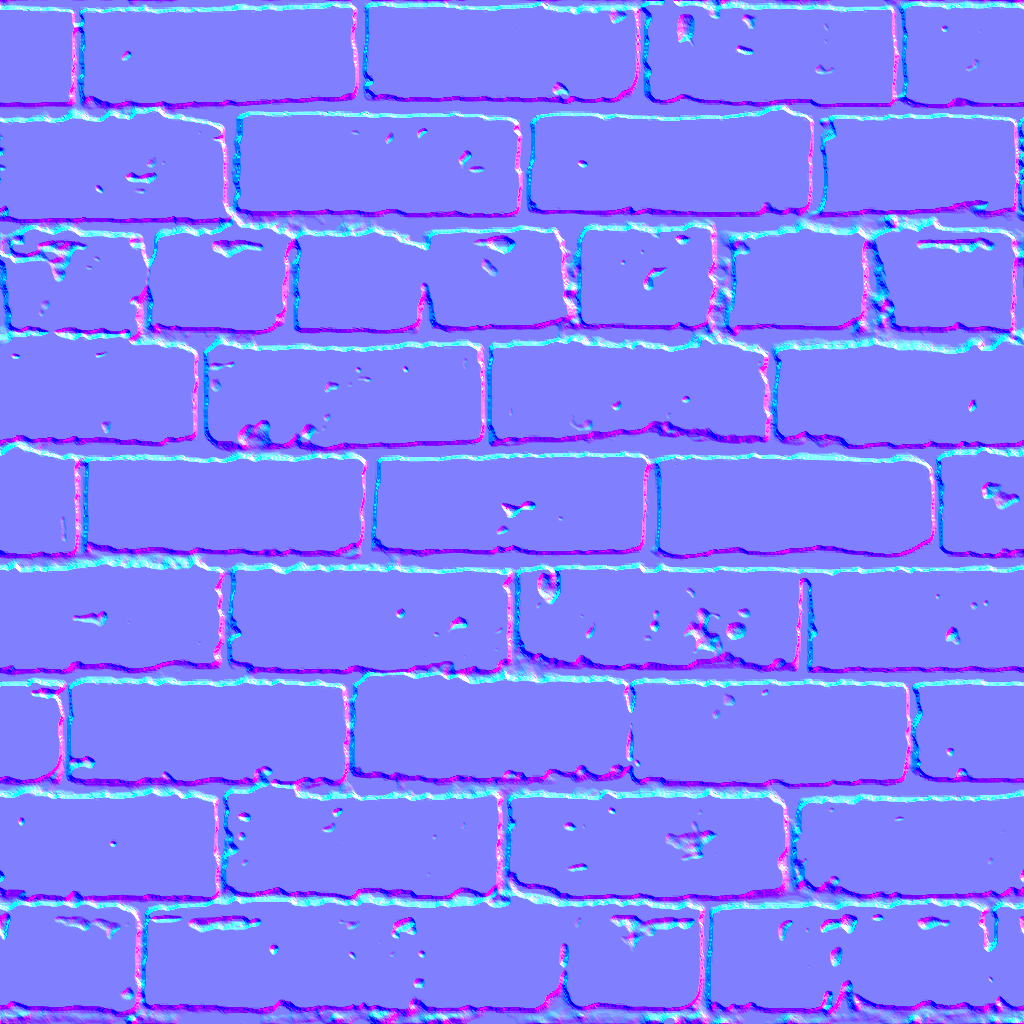
\includegraphics[width=0.5\linewidth]{intructions/Brick001_n.png}
 		\centering
 		\captionof{figure}{The normal map that I created}
 		\label{fig:test19}
 	\end{minipage}
 	\begin{minipage}{.33\textwidth}
 		\centering
 		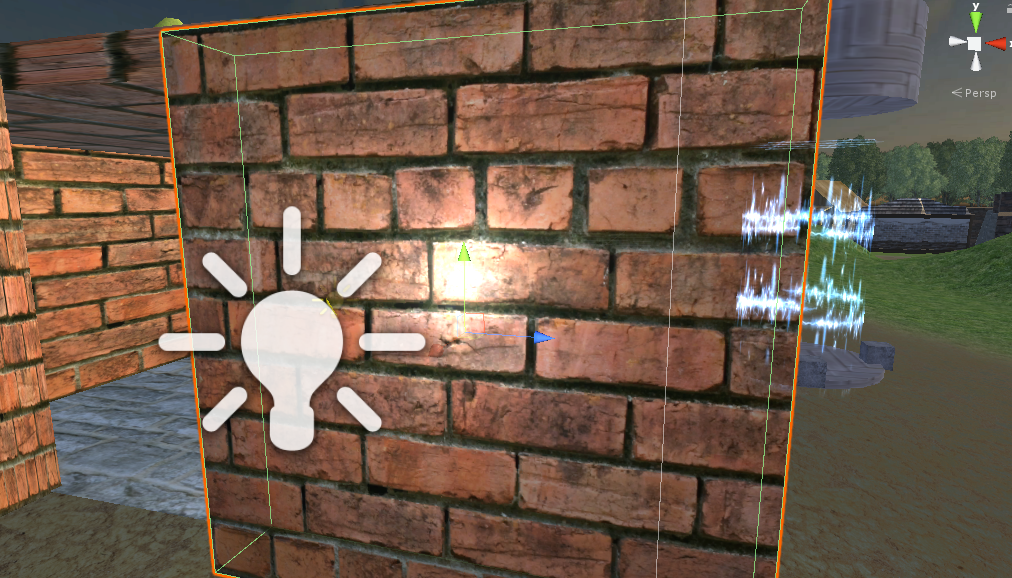
\includegraphics[width=1\linewidth]{intructions/without_normalmap.png}
 		\centering
 		\captionof{figure}{Without normal map}
 		\label{fig:test20}
 	\end{minipage}
 	\begin{minipage}{.33\textwidth}
 		\centering
 		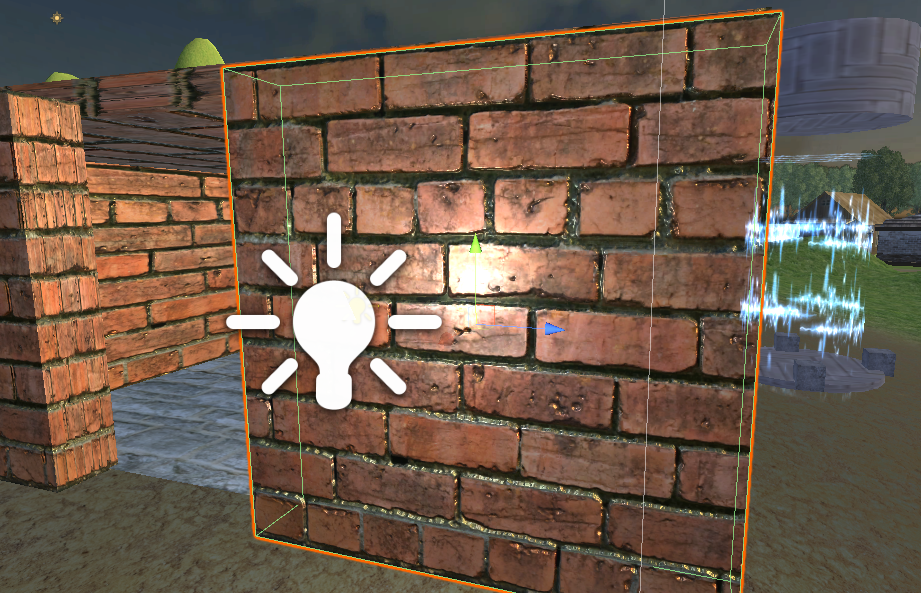
\includegraphics[width=1\linewidth]{intructions/with_normalmap.png}
 		\captionof{figure}{With normal map applied}
 		\label{fig:test21}
 	\end{minipage}
 \end{figure} 

\begin{itemize}
	\item \bfseries Occlusion map	 	
\end{itemize}
The occlusion map will determine which area are inherently darkened to simulate shadow, anywhere is white will not receive darkening, anywhere that's black or gray will receive darkening. For this map, as I can't find a proper way, algorithm to actually generate a true occlusion map from just a 2d texture, so I decided to write a C\# script outside Unity to make an occlusion map, because in Unity, there is no System.Draw library for editing the texture.
\newpage
\begin{figure}[h]
	\centering
	\raisebox{-25mm}[0pt][0pt]{
		\begin{minipage}{.4\textwidth}
			\centering
			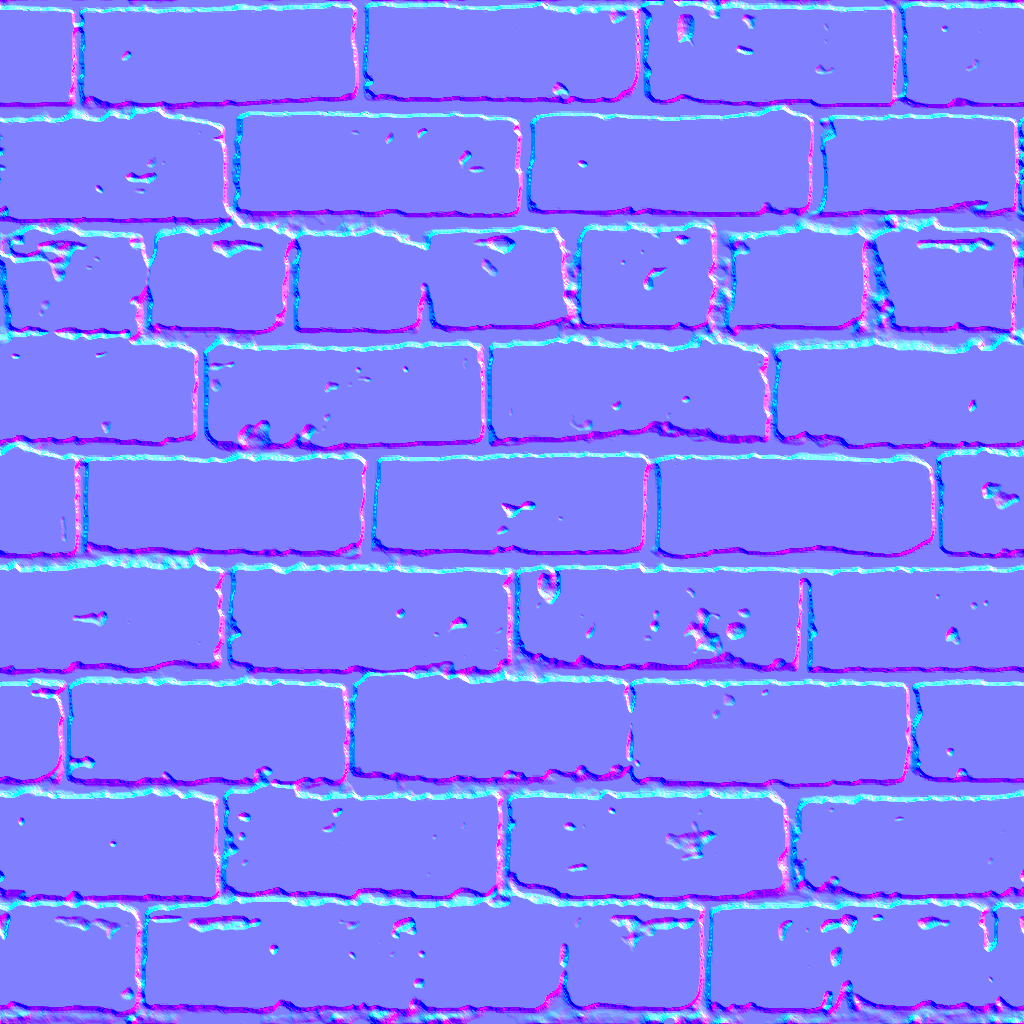
\includegraphics[width=0.8\linewidth]{intructions/Brick001_n.png}
			\centering
			\captionof{figure}{The normal map}
			\label{fig:test22}
		\end{minipage}
		\begin{minipage}{.4\textwidth}
			\centering
			
\includegraphics[width=0.8\linewidth]{intructions/Brick001_occ.png}
			\centering
			\captionof{figure}{Occlusion map after I created using C\# script}
			\label{fig:test23}
		\end{minipage}
	}
\end{figure}
\vspace{5.5cm}
From 2 images above, the purple color, with RGB value of (0.5, 0.5, 1) as base color, with z direction being up as the blue channel. The reason the values in the textures are treated as having been halved, with 0.5 is because from the equation above I mentioned in above section, is divided by 2 when normalizing the height value. In the normal map texture, I found out that the bluish color and the deep purple one is actually the direction of the light shining on the surface of the texture, as the deep purple is behaved as opposite direction with the bluish one. When convert the texture into grey-scale image by getting red, green, blue color and divided by 3, the light blue area will turn into white color, the purple one will turn into dark-grey color, which behave almost like an occlusion map. To make sure that the surface(or the light grey area) will not too dark when applying occlusion map, I've lighten up the texture a bit by using ControlPaint.Light function just like in figure 23. 
\begin{figure}[h]
	\begin{minipage}{.4\textwidth}
		\centering
		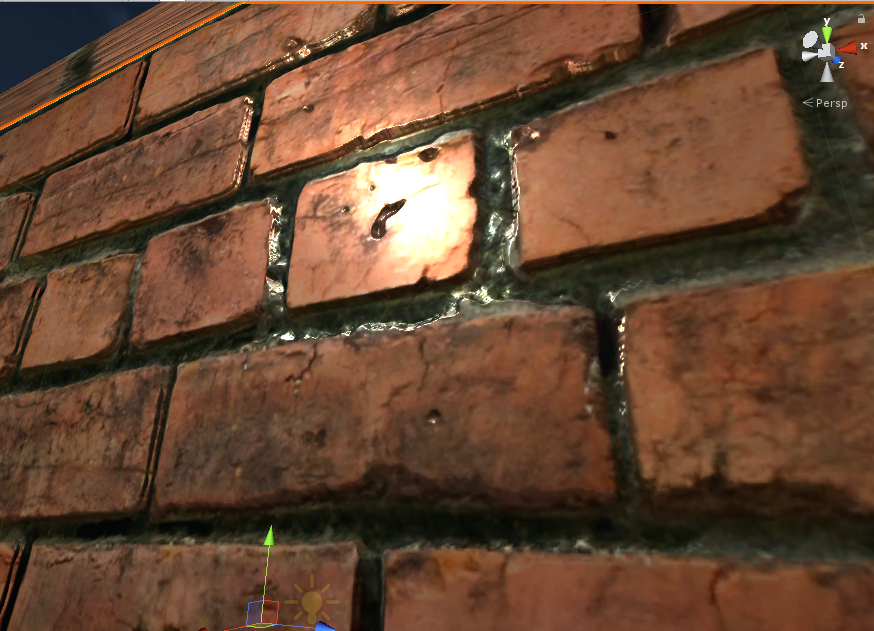
\includegraphics[width=1\linewidth]{intructions/without_occlusion.png}
		\centering
		\captionof{figure}{without occlusion}
		\label{fig:test24}
	\end{minipage}
	\begin{minipage}{.45\textwidth}
		\centering
		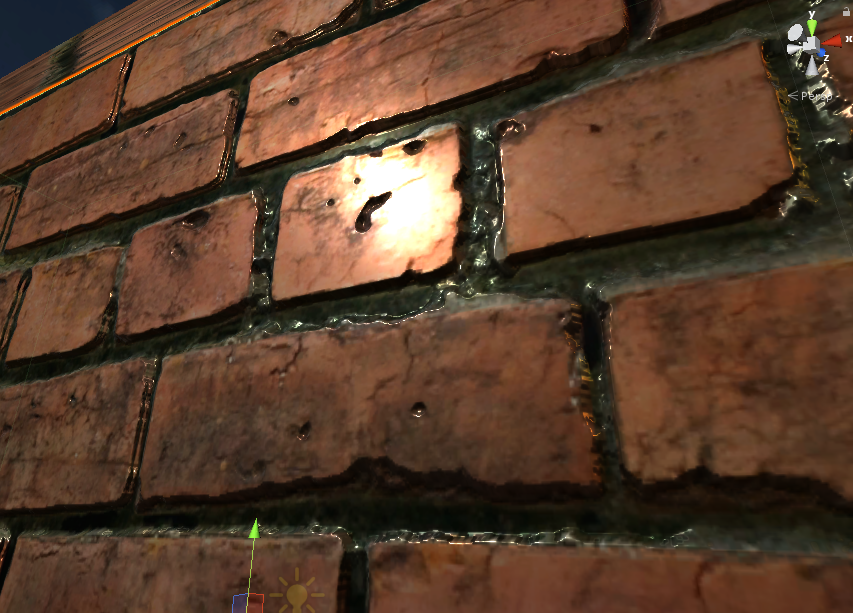
\includegraphics[width=0.9\linewidth]{intructions/with_occlusion.png}
		\centering
		\captionof{figure}{with occlusion being applied}
		\label{fig:test25}
	\end{minipage}
 
\end{figure}
It's quite hard to see the difference, but in the right side, at the bottom of the brick, it's darker than the left side as if there is a shadow there.

\paragraph{Lighting}
Lighting is an essential part of every scene. In Unity, while the mesh, textures define the shape, the look of an object, the lights will define the color, the mood of a 3D environment. Lights can be added into the scene just by going to {\bfseries GameObject -> Light} menu. In the menu, we can choose any form of light. Once the light has been added into the scene, we can adjust the properties of the light to the way we want in the inspector, there are many different options within the Light Component. 
\newpage
\begin{figure}[h]
	\centering
	\raisebox{-25mm}[0pt][0pt]{
		\begin{minipage}{.4\textwidth}
			\centering
			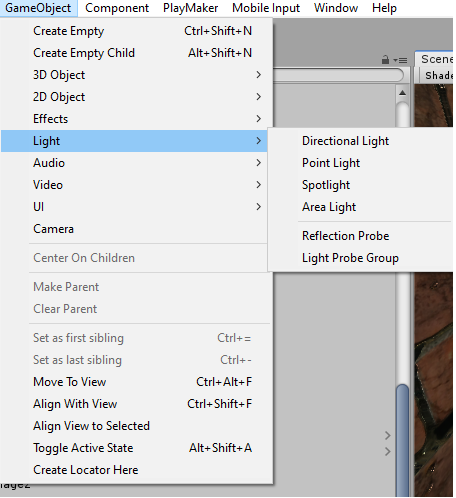
\includegraphics[width=0.8\linewidth]{intructions/choose_light.png}
			\centering
			\captionof{figure}{Light section}
			\label{fig:test26}
		\end{minipage}
		\begin{minipage}{.45\textwidth}
			\centering
			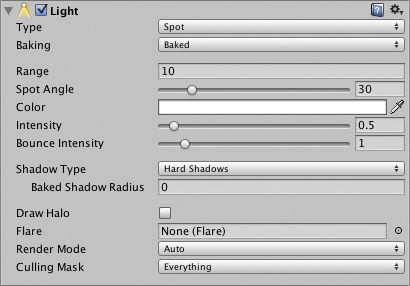
\includegraphics[width=1.2\linewidth]{intructions/light_properties.png}
			\centering
			\captionof{figure}{Light properties}
			\label{fig:test27}
		\end{minipage}
	}
\end{figure}
  \vspace{5.5cm}
  Just by simply changing the color of a light, this can give a whole different mood to the scene.
  \begin{figure}[h]
  	\begin{minipage}{1\textwidth}
  		\centering
  		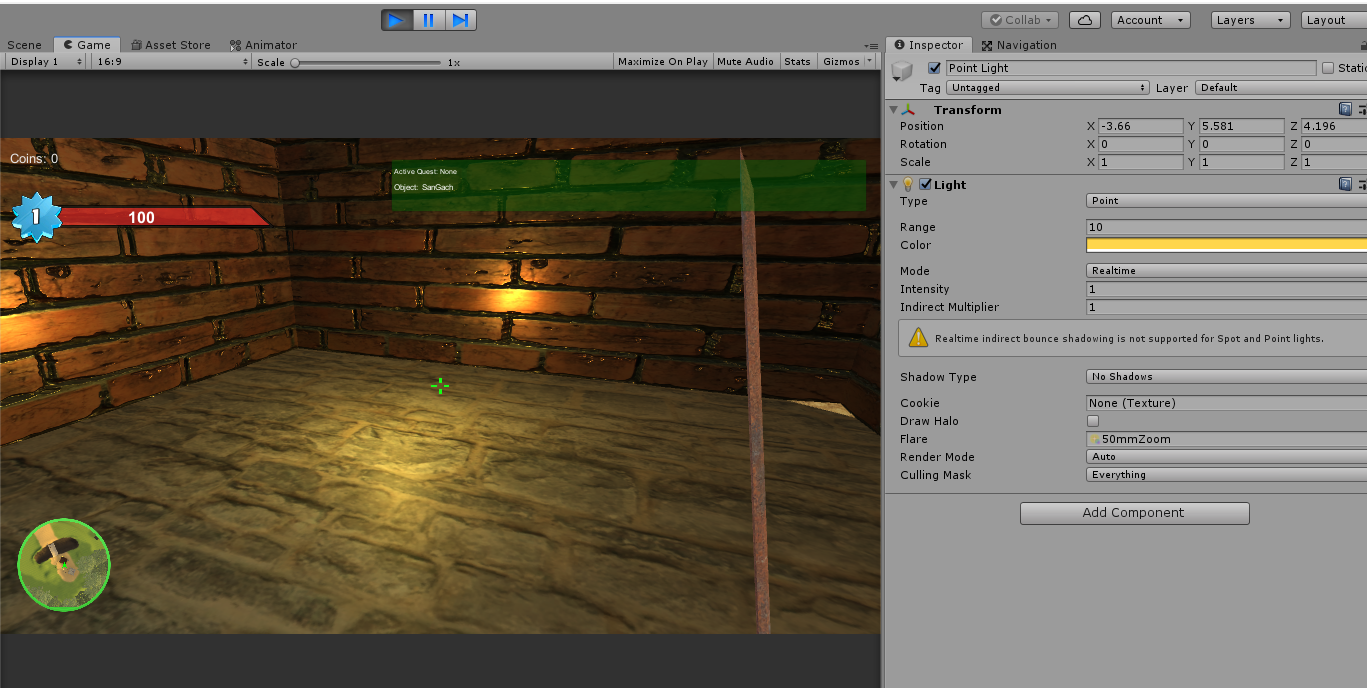
\includegraphics[width=0.8\linewidth]{intructions/change_light_color.png}
  		\centering
  		\captionof{figure}{Changing light color}
  		\label{fig:test28}
  	\end{minipage}
  \end{figure} \\
 However, lighting in Unity also includes realtime GI or global illumination, illumination means lighten up. GI is a general name for a group of methods and algorithms to add more realistic lighting into the scene, like how the like is bounce off surface onto other surfaces, instead of just limited to the light that hit the surface directly. 
 \begin{figure}[h]
 	\begin{minipage}{1\textwidth}
 		\centering
 		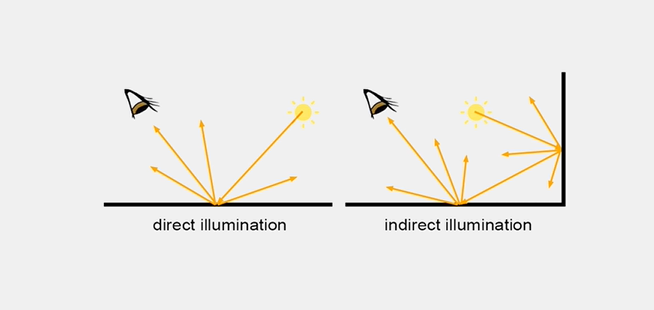
\includegraphics[width=0.8\linewidth]{intructions/light_categlories.png}
 		\centering	
 		\captionof{figure}{(Image from number \cite{Youtuber}, youtube channel Brackeys)}
 		\label{fig:test270}
 		\end{minipage}
 	\end{figure}
 \\[0.05cm]
 In computer graphic, this act of light bouncing around into two categories: direct illumination and indirect illumination. Direct lighting is when light gets send out from a light source, bounces and then reaches the eye (or the camera). Indirect lightning is when light bounces off multiple surfaces before hitting the eye, light will keep bouncing until it get fully absorbed. From the figure 26, all the type of light from Light section, like directional light, point light, etc.. they are all direct lights because they're all light source. When defining about indirect lighting, which mean every kind of light that's not directly point anywhere from the scenes, but by going to Window -> Rendering -> Lighting and look at environment lighting section, that's a great example of indirect lighting and so GI. And this's actually when GI basically comes to play, and GI will take care of direct lighting and indirect lighting that reflect from surfaces meaning it helps illuminating the scene more realistically. 
 \begin{figure}[h]
 	
 \end{figure}
 Without GI enabled, we cannot see any light bounce at all, even the light source is directly pointing at the sphere. With GI enabled, the room is now become a bit brighter , with a bit of light bouncing to the ceiling. The way the GI works, is that when the light travel through the gap that seen from the image above, and then the photon that travel from the light source will carry the values of surface that hit to the next surface. And with that way which can explain the reason why we can see the green light on the ceiling, that's the light that inherit from the green cube and blue sphere. 
  \begin{figure}[h]
 	\begin{minipage}{1\textwidth}
 		\centering
 		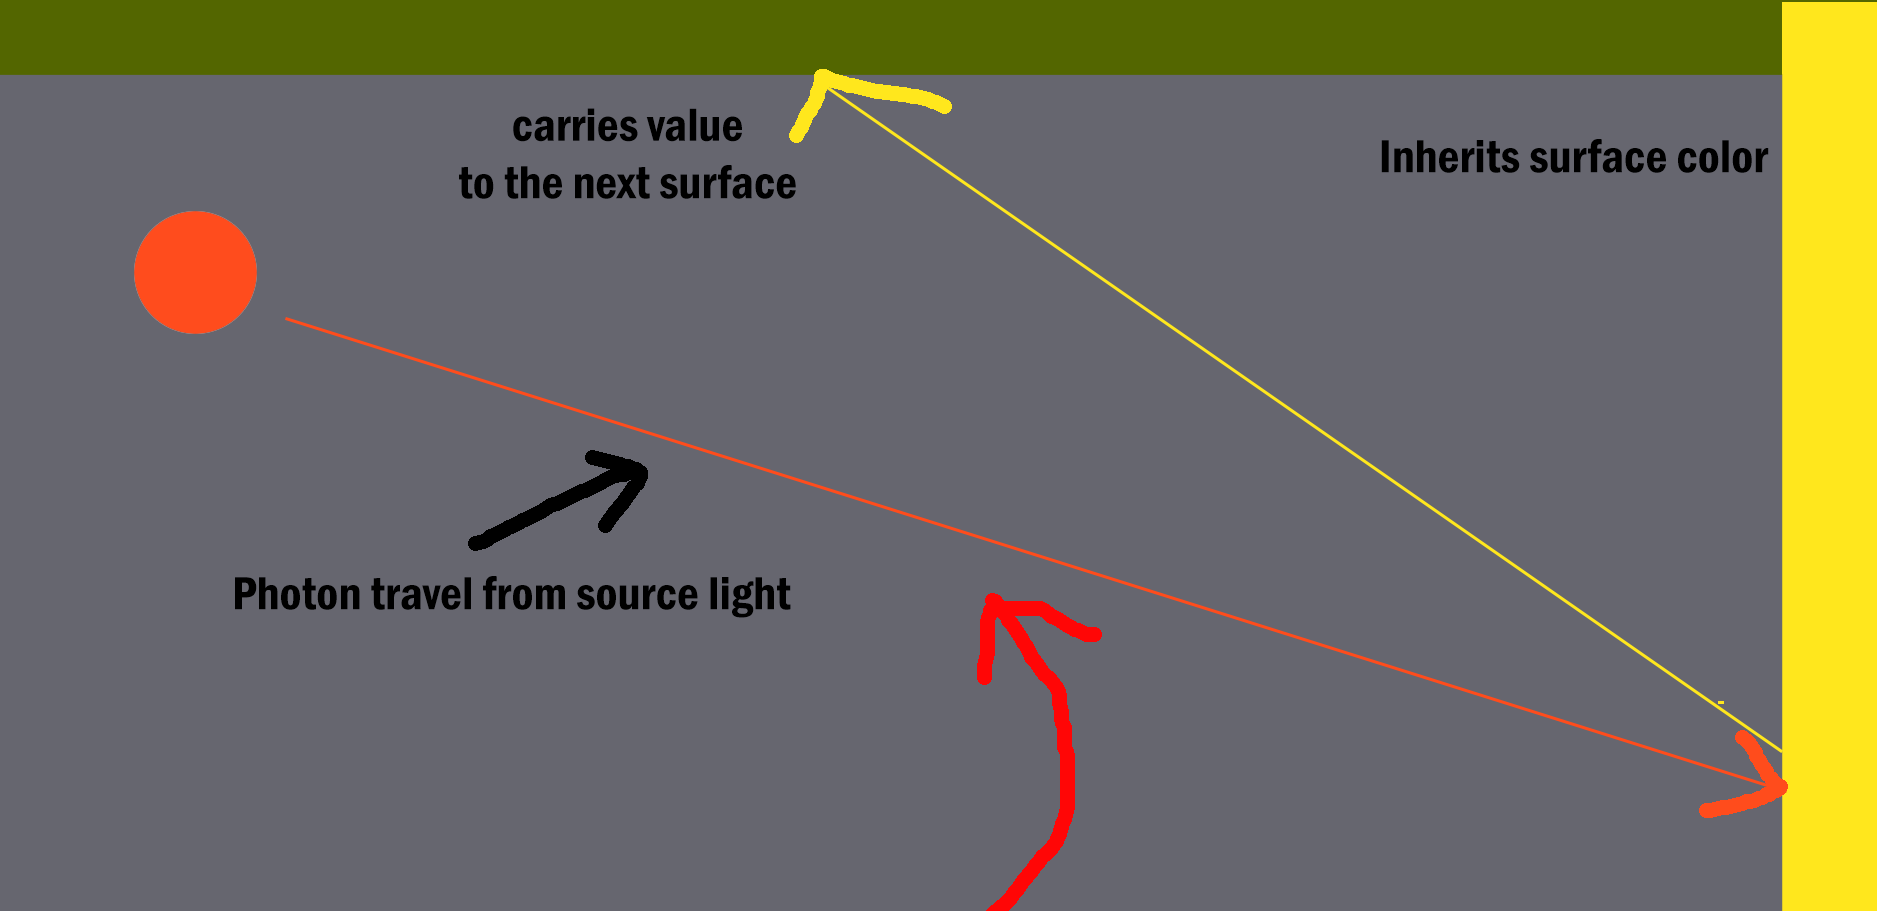
\includegraphics[width=0.8\linewidth]{intructions/How_light_works.png}
 		\centering
 		\captionof{figure}{GI technique}
 		\label{fig:test271}
 	\end{minipage}
 \end{figure}
\\[0.05cm]
 In Unity, it provides two techniques for pre computing GI: Baked GI and pre-computed real-time GI. The Baked one is pre-computed and will save a ton of processing power, and this only work if all the objects, light-sources in the scene are static. Whereas real-time is exactly lighting calculated in real-time, per frame, which means light and shadow positions can change over time when an object or light source is moving. Depending on each object and light source, we select the appropriate GI method. For the sunlight (the light that shines the whole scene), I set the mode to real-time because there are still some moving objects like the player, the NPC, etc... and for the light like the room light, I set it to baked mode. A combination of baked and realtime lights can help maintain performance. To enable GI mode, all I have to do is go to window -> rendering -> lighting setting, here's the properties that I set for making the light looks more realistic. The reason I have to enable both realtime and baked GI is because I have both baked and realtime light in the scene.
 \begin{figure}[h]
 	\raisebox{-50mm}[0pt][0pt]{
 	\begin{minipage}{1\textwidth}
 		\centering
 		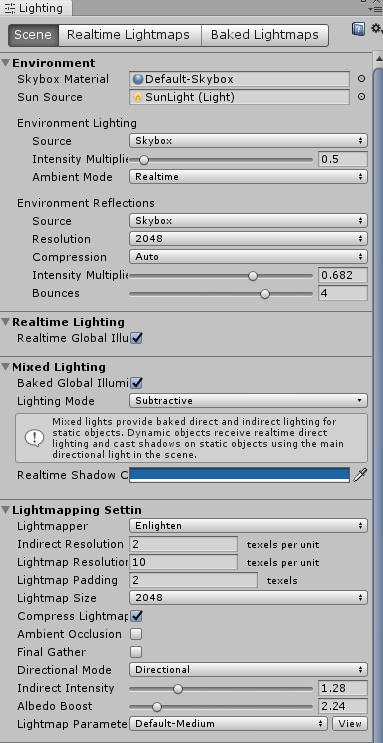
\includegraphics[width=0.3\linewidth]{intructions/lighting_setting.png}
 		\captionof{figure}{Light setting}
 		\centering
 	\end{minipage}
}
 \end{figure}
\vspace{100mm}
 However, there are currently limitations of GI so both baked and pre-computed real-time GI in Unity have the limitation that only objects in the scene that set to static can be included that means moving objects cannot bounced light onto other objects and vice versa, but still they can pick up bounced light from static object using light probes. Light Probes can be created by going to GameObject -> Light -> Light probe groups.
 
 \paragraph{Shader} \vspace{-0.2cm}
 \subparagraph{Shader overview} ~\\[0.1cm]
 A shader is basically a type of program that's executed on the GPU, it can simulate how a particular surface responds to light. A shader will decide how the scene in a game will look. The diagram below respresents three different entities, show rendering workflow of Unity, how it can use the shader. 
 \begin{figure}[h]
 		\begin{minipage}{1\textwidth}
 			\centering
 			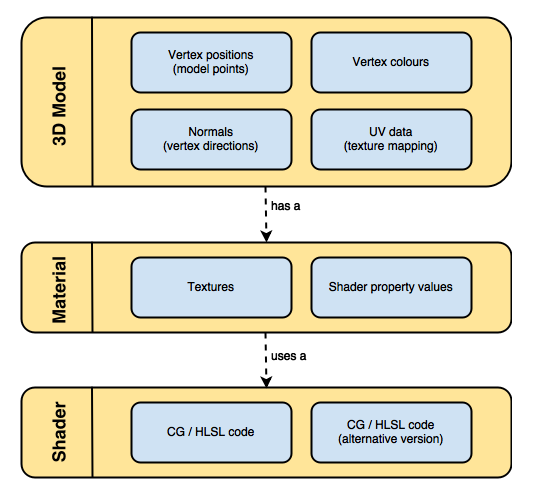
\includegraphics[width=0.4\linewidth]{intructions/Shader_workflow.png}
 			\centering
 		\end{minipage}
 \end{figure}
\newpage
   Model cannot be rendered without a material, and material are wrappers which contain a shader and values for its properties, different material can share the same shader. In Unity, shaders are written in a custom environment called ShaderLab, which can be customized a lot about how the material will use a shader. Normally, Unity does come with a build-in shader called standard shader, which I was used in the whole section above for showing my demo. In a shader file, there are 2 main components: Properties and subshader. In the properties and subshader function, the parts where to define variables are the shaderlab, which is almost like the front-end development, they're all written in CG/HLSL high-level language. \\
   When writing a shader, in the properties tab, we can define any value  so that we can change them in Unity's inspector later. In a subshader, it can have multiple pass command, each pass command is the combination of vertex, fragment function. In some situation like the object needs to have multiple textures or color, multiple pass command will be used here. A shader can also have multiples subshader, especially the game/app for multiple-platform, as the gpu will only find compatible shader, render to the object, because not all the devices function all the same , they also have different hardware configuration, a shader with multiple-shader will take account here. In general, the structure of a shader in Unity will look like this: 
   \begin{lstlisting}
   Shader "ABC/XYZ" {
   	Properties{
   		//Difine variable here	
   	}
   	SubShader {
   		{[Name and Tags] [RenderSetup]}
   		Pass {
   		{[Name and Tags] [RenderSetup]}
		   CGPROGRAM
		   ENDCG
   		}
  	 }
   }
   \end{lstlisting}
  The properties of the shader are somehow equivalent to the public fields in a C\# script, they will appear in the inspector of a material, can be editable. The subshader is the section that use to write the code, a shader script can have multiple sections, one after other, they contain the actual intructions for the GPU. When defining the properties , the material inspector will look like this: 
   \begin{figure}[h]
  	\begin{minipage}{1\textwidth}
  		\centering
  		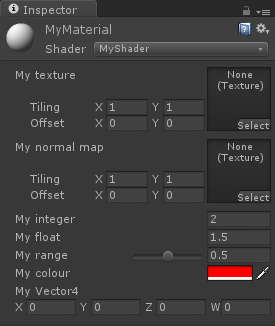
\includegraphics[width=0.2\linewidth]{intructions/Inspector_material.png}
  		\centering
  	\end{minipage}
  \end{figure}
But, this is not enough to use the properties. This section is only use to give access to hidden variables within subshader section. They still need to define in the subshader section, which is the actual body. 
\begin{lstlisting}
SubShader
{
// Code of the shader
// ...
sampler2D _MyTexture;
sampler2D _MyNormalMap;

int _something;
float _something;

// Code of the shader
// surface shader code or vertex and fragment shader
}
\end{lstlisting}
What I mentioned above in the code example above, Unity supports two different types of shaders: surface shader, fragment and surface shader.
\begin{itemize}
	\item[--] The surface shader is used whenever the material needs to be simulated to be affected by lights in a realistic way. Surface shaders hide the calculations of how light is reflected and allows to specify “intuitive” properties such as the albedo, the normals, the reflectivity and so on in a function called surf. These values are then plugged into a lighting model which will output the final RGB values for each pixel. The surf function contains both the vertex and fragment, the pass command cannot be used with surf function.
\end{itemize}
 	The Cg code of a surface shader will looks like this: 
 	\begin{lstlisting}
 	#pragma surface surf Lambert //This is Lambertian lighting model
 	sampler2D _MainTex; // The input texture
 	
 	struct Input {
 	float2 uv_MainTex;
 	};
 	
 	void surf (Input IN, inout SurfaceOutput o) {
 	o.Albedo = tex2D (_MainTex, IN.uv_MainTex).rgb;
 	}
 	\end{lstlisting}
 	
 \begin{itemize}
 	\item[--] Vertex and fragment shader work close to the way the GPU renders triangles, and have no built-in concept of how light should behave, it's a low-level shader than the surface shader. A vertex and fragment shader's structure in Unity will look like this:
 		\begin{lstlisting}
 	SubShader
 	{
 		Tags { "RenderType"="Opaque" }
 		LOD 100
 		
 		Pass
 		{
 		CGPROGRAM
 		#pragma vertex vert
 		#pragma fragment frag
 		
 		#include "UnityCG.cginc"
 		
 		struct appdata
 			{
 			};
 		
 		struct v2f
 			{
 			};
 			
 		sampler2D _MainTex;
 		float4 _MainTex_ST;
 		
 		v2f vert (appdata v)
 			{
 			}
 		
 		fixed4 frag (v2f i) : SV_Target
 			{
 			}
 		ENDCG
 		}
 	}
 \end{lstlisting}
 \end{itemize}
The geometry of the model will past through a function call vert which can alter its vertices. And then, individual triangles of the geometry are passed through another function called frag which will decided the final RGB color for every pixel. This shader is usually use for 2D effects, post processing and special 3D effect which are too hard to be expressed as surface shader. And from the image below, here's a shader flow for vertex and fragment shader in Unity works. Object data is actually the textures of a model that should be prepared before.
   \begin{figure}[h]
	\begin{minipage}{1\textwidth}
		\centering
		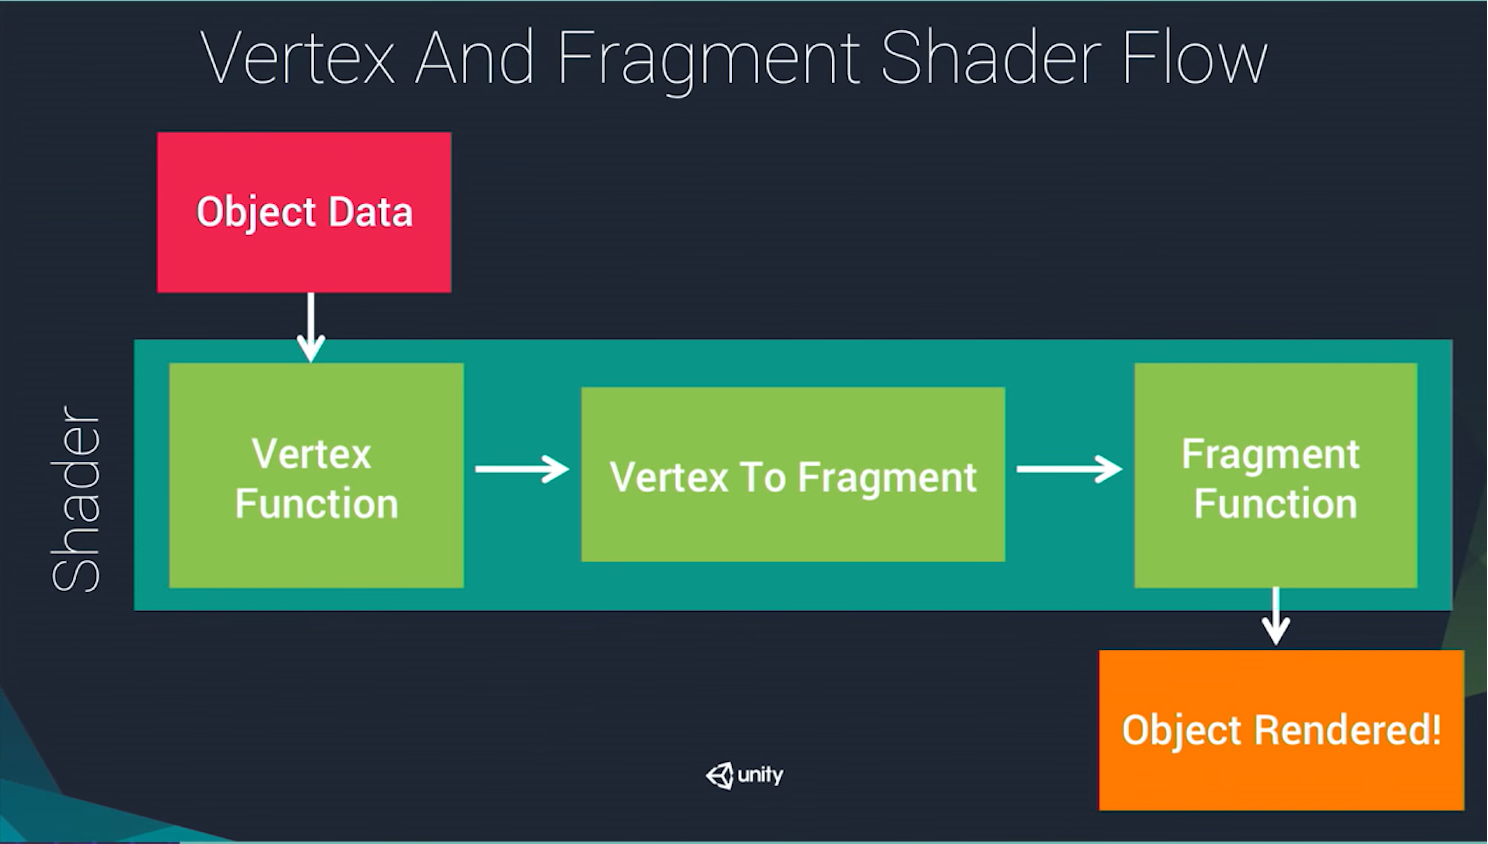
\includegraphics[width=0.55\linewidth]{intructions/vertex_fragment_flow.png}
		\captionof{figure}{Vertex and fragment Shader flow}
		\label{fig:test29}
		\centering
	\end{minipage}
\end{figure}
From Unity 2018 version or later, it does comes with shadergraph to be able to make a shader without actually coding but the shadergraph is still in beta stage , have lots of bug so I decided to make a custom shader manually. As I don't have a lot of time in this project, so I'll only write a very basic one. 
 \subparagraph{Apply shader on 3D mesh} ~\\[-0.8cm]
 \begin{itemize}
 	\item \bfseries Fresnel effect
 \end{itemize}
   This is the effect that many people use in a game. With fresnel, I can darken, lighten the outline of an object. For this shader, I'll use on my character, with surface shader because I need my character's surface to react with. \\[0.01cm] According to Unity's document, the fresnel's equation is calculated as: \\ {\bfseries Out = pow((1.0 - saturate(dot(normalize(Normal), normalize(ViewDir)))), Power) }, where the saturate function is to clamp the variable to be between 0 and 1 \\
   The normal surface is defined by normal vectors like this picture: 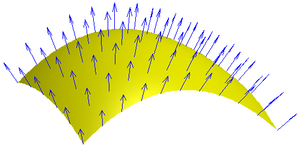
\includegraphics[width=0.3\linewidth]{Surface_normal.png}
   And for the view direction, in order to get this view, all I have to do is defining float3 viewDir from the struct Input in the surface shader, where the float3 is a variable with 3 dimension, the same as float2 and float. 
   
   After writing a fresnel shader base on the following equation, the material will looks like this:
    \begin{figure}[h]
    	\raisebox{-21mm}[0pt][0pt]{
    	\begin{minipage}{.4\textwidth}
    		\centering
    		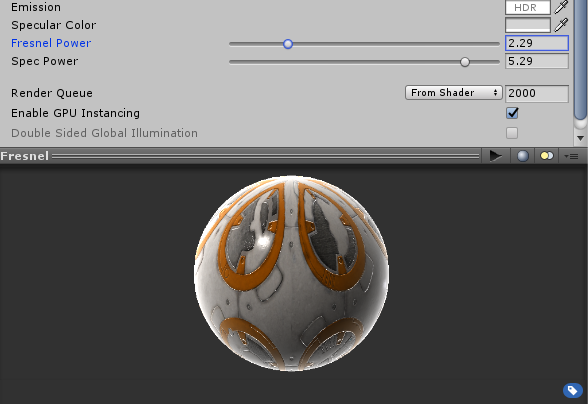
\includegraphics[width=1\linewidth]{intructions/fresnel_effect.png}
    		\centering
    	\end{minipage}
    }
    \end{figure}
\newpage
   \begin{lstlisting}
   struct Input
   {
   float4 color : COLOR;
   float2 uv_MainTex;
   float2 uv_BumpMap;
   float3 worldNormal;
   float3 viewDir;
   INTERNAL_DATA
   };   
   void surf(Input IN, inout SurfaceOutput o)
   {
   // Albedo comes from a texture tinted by color
   fixed4 c = tex2D(_MainTex, IN.uv_MainTex) * _Color;
   o.Albedo = c.rgb * _LightColor0.rgb;
   o.Alpha = c.a * _Color.a;
   o.Normal = UnpackNormal(tex2D(_BumpMap, IN.uv_BumpMap));
   float fresnel = dot(normalize(o.Normal), normalize(IN.viewDir)); //The reason I use o.Normal here instead of IN.worldNormal is because I have applied the normal texture in the object.
   fresnel = pow(saturate(1 - fresnel), _FresnelPower);
   o.Emission = fresnel * _Emission;
   }
   ENDCG							  
   } 
   FallBack "Diffuse"
   }
   \end{lstlisting}
  With this , I can make the fresnel effect stronger or weaker just by adjusting the exponent of it, rendering nice effect for my character. For me, the value from 0 to 10 is enough, fits in this shader.
   \begin{itemize}
  	\item \bfseries Glass shader
  \end{itemize}  
  	The fresnel effect above can also be used to create a glass shader. First of all, I am going to define alpha:fade which is going to make the object be able to see inside. When creating a shader, Unity already implement for us the smoothness, metallic value so I just need to increase both of the value to 1 in order to make the object reflective. After that, the object still doesn't look like a glass, in order to get the glass look, this is when the fresnel effect comes to play. Same as before, but this time, instead of multiplying the equation with o.Emission, I'll multiply it with o.Alpha, to get the glass look, as o.Alpha alter the transparent of the object.
  	\begin{figure}[h]
  		\begin{minipage}{.5\textwidth}
  			\centering
  			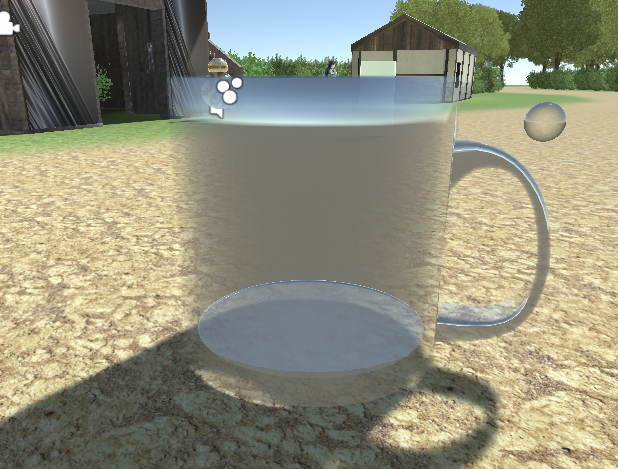
\includegraphics[width=0.7\linewidth]{intructions/whole_surface.png}
  			\centering
  			\captionof{figure}{Without fresnel}
  			\label{fig:test30}
  		\end{minipage}
  		\begin{minipage}{.5\textwidth}
  			\centering
  			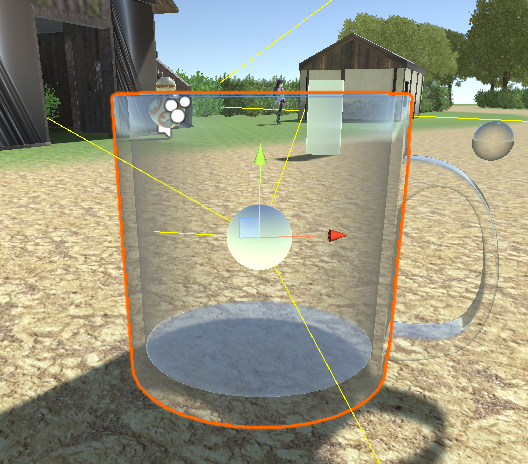
\includegraphics[width=0.6\linewidth]{intructions/from_edge.png}
  			\centering
  			\captionof{figure}{With fresnel}
  			\label{fig:test31}
  		\end{minipage}
  		
  	\end{figure}
     \begin{lstlisting}
     void surf (Input IN, inout SurfaceOutputStandard o)
     {
	     // Albedo comes from a texture tinted by color
	     fixed4 c = tex2D (_MainTex, IN.uv_MainTex) * _Color;
	     o.Albedo = c.rgb * _ColorMult;
	     // Metallic and smoothness come from slider variables
	     o.Metallic = _Metallic;
	     o.Smoothness = _Glossiness;
	     //Getting the reflection
	     float border = 1- saturate((dot(normalize(IN.worldNormal), normalize(IN.viewDir))));
	     float alpha = pow(border, _Reflective);
	     o.Alpha = ((c.a)  * alpha);
     }
      \end{lstlisting}
      But, this will only get the reflection from the empty space, not in the scene itself, so finally, to get the reflection from all objects around it, a reflection probe need to be added in order to make the glass looks more realistic.
      \begin{figure}[h]
      	\begin{minipage}{1\textwidth}
      		\centering
      		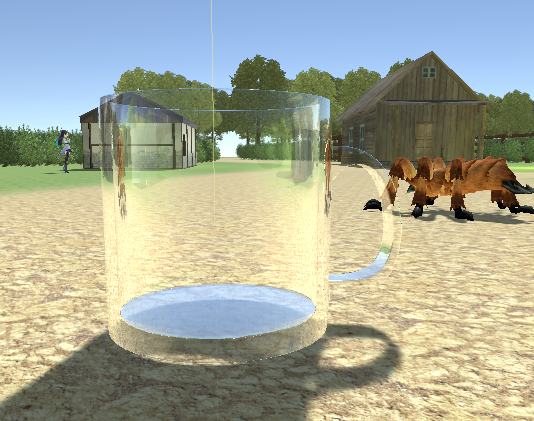
\includegraphics[width=0.4\linewidth]{intructions/reflection_probe.png}
      		\centering
      		\captionof{figure}{with reflection probe}
      		\label{fig:test32}
      	\end{minipage}      	
      \end{figure}
  \begin{itemize}
 	\item \bfseries Object always visible 
  \end{itemize}
This shader will make an object always be see-through, be rendered whenever it's behind any object or not, so in this section, I am going to write a fragment/vertex shader instead of surface shader. This shader's going to have 2 passes, the first pass is for rendering the shape of an object if it's behind something, the second one is for rendering object texture. Because the pass order in the shader does matter so I will make the color to render first. 

\begin{lstlisting}
Pass
{
CGPROGRAM
#pragma vertex vert
#pragma fragment frag

#include "UnityCG.cginc"
struct appdata
{
	float4 vertex : POSITION;
	};
	struct v2f
	{
		float4 vertex : SV_POSITION;
	};
	
	sampler2D _MainTex;
	float4 _Color;
	
	v2f vert(appdata v)
	{
		v2f o;
		o.vertex = UnityObjectToClipPos(v.vertex);
		return o;
	}
	
	fixed4 frag(v2f i) : SV_Target
	{
		return _Color;
	}
	ENDCG
}	
\end{lstlisting}
The first pass will return the color depend on which color I choose 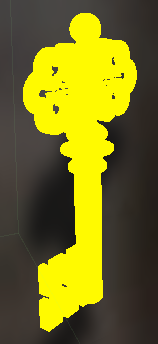
\includegraphics[width=0.04\linewidth]{intructions/color_alwaysvisible.png}, but the object will not be visible if there is an object in front of it. To do that, I just simply add Ztest always within the pass command, this function will always render the pixel of this object no matter how matter which pixel is closer or further than the camera. And as a result, the yellow color that I choose still be rendered even it's behind the wall:  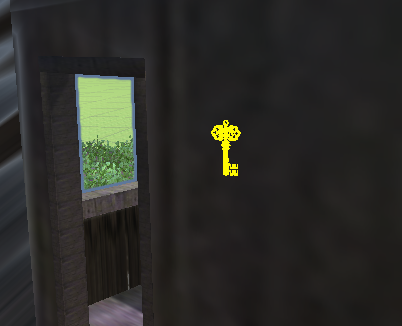
\includegraphics[width=0.3\linewidth]{intructions/Behind_overlay.png}
For second pass, I will put the texture into my object:
\begin{lstlisting}
	struct appdata
	{
		float4 vertex : POSITION;
		float2 uv : TEXCOORD0;
	};
	
	struct v2f
	{
		float2 uv : TEXCOORD0;
		float4 vertex : SV_POSITION;
	
	};
       v2f vert (appdata v)
      {
	      v2f o;
	      o.vertex = UnityObjectToClipPos(v.vertex);
	      o.uv = TRANSFORM_TEX(v.uv, _MainTex);
	      return o;
      }
      
      fixed4 frag (v2f I) : SV_Target
      {
	      // sample the texture
	      fixed4 col = tex2D(_MainTex, I.uv);
	      return col;
      }
      ENDCG
\end{lstlisting}
\begin{figure}[h]
	\begin{minipage}{.4\textwidth}
		\centering
		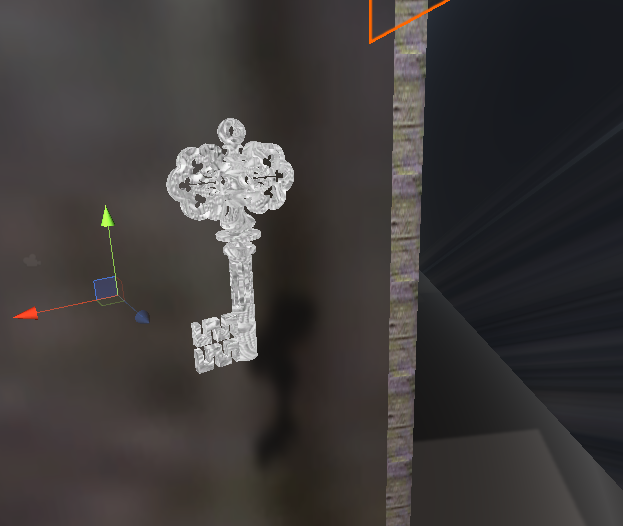
\includegraphics[width=0.7\linewidth]{intructions/key_with.png}
		\centering
	\end{minipage}
	\begin{minipage}{.45\textwidth}
		\centering
		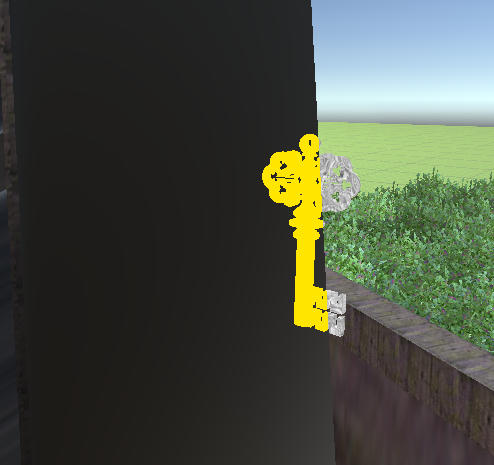
\includegraphics[width=0.6\linewidth]{intructions/key_with2.png}
		\centering
	\end{minipage}
\end{figure}
At this moment, the object doesn't react to the light yet, the surface shader is also used here and combined with the vertex/fragment shader in order to make the lighting work.

\begin{lstlisting}
CGPROGRAM
// Physically based Standard lighting model, and enable shadows on all light types
#pragma surface surf BlinnPhong fullforwardshadows
#include "UnityCG.cginc"
// Use shader model 3.0 target, to get nicer looking lighting
#pragma target 3.0
sampler2D _MainTex;
struct Input
{
	float4 color : COLOR;
	float2 uv_MainTex;
};
void surf(Input IN, inout SurfaceOutput o) {
	o.Albedo = tex2D(_MainTex, IN.uv_MainTex).rgb;
}
ENDCG
\end{lstlisting}
\newpage
~
	 \begin{figure}[h]
	
			\begin{minipage}{1\textwidth}
				\centering
				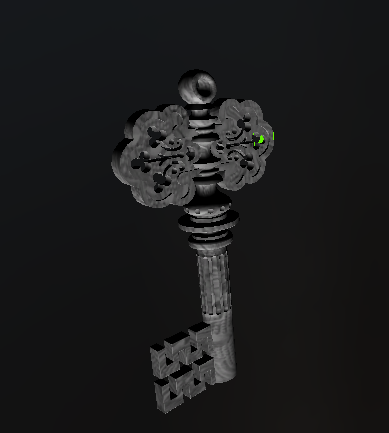
\includegraphics[width=0.3\linewidth]{intructions/light_react.png}
				\captionof{figure}{Light react}
				\centering
			\end{minipage}
	\end{figure}
\subparagraph{Post processing} ~\\
Post processing is a shader that instead of applying to an object, it will be applied directly into the camera, the effect will be being rendered to the whole screen, within the window box. Just like other shaders that applied on an object, the structure is the same, but post processing doesn't use surface shader as the camera only render 2d images, show them to the computer monitor.
\begin{itemize}
	\item \bfseries Dizzy effect 
\end{itemize} 
 This effect will make the entire scene looks like it's swinging. But first off all, we will need to implement graphics.blit in C\# code to render the shader into the screen. In the shader file, the fragment function is where it draw all the color into the screen. The window which we are able to see the scene is the clip point, the clip point is defined by the uv coordinate, range from (0,1), so in order to achieve the effect on screen, we'll need to alter the u, v coordinate. To do that,we just add a simple mathematic equation with I.uv : 
 \begin{lstlisting}
  struct appdata
 {
 float4 vertex : POSITION;
 float2 uv : TEXCOORD0;
 };
 struct v2f
 {
 float2 uv : TEXCOORD0;
 float4 vertex : SV_POSITION;
 };
 fixed4 frag (v2f I) : SV_Target
 {
 fixed4 col = tex2D(_MainTex, I.uv + float2(0, sin (I.vertex.x/80 * _Time[1]/20)/10 ));
 return col;
 }
 \end{lstlisting} 
 This equation will make the scene looks like it's be curved with the sin wave, on the x position, where I.vertex is the output position to the world space. As a result, the scene will looks like this: 
 \newpage
 ~
 \begin{figure}[h] 
 	\begin{minipage}{1\textwidth}
 		\centering
 		\includegraphics[width=0.7\linewidth]{intructions/dizzy.png}
 		\centering
 		\captionof{figure}{Dizzy effect}
 		\label{fig:test33}
 	\end{minipage}      	
 \end{figure}
\begin{itemize}
	\item \bfseries Post-processing stack 
\end{itemize} 
From Unity 2018 or later, it has built-in tool which is called post-processing stack, mainly for post-processing effect.  It’s applies effects after the main processing pipeline and enhances the overall look of a scene. So, with this tool, we'll gonna make the scene looks more fancy, brilliant. 
First of all, we'll need to configure some settings by going to {\bfseries Edit -> Project Settings -> Quality}. 
  \begin{figure}[h] 
 	\begin{minipage}{1\textwidth}
 		\centering
 		\includegraphics[width=0.5\linewidth]{intructions/quality_setting.png}
 		\centering
 		\captionof{figure}{Quality setting}
 		\label{fig:test34}
 	\end{minipage}      	
 \end{figure}
For the anti-aliasing, I'll only set to 2x, even better if it's turned off. When set too high, it may decrease performance, my computer might not be able to handle this. Anti-aliasing is for getting rid of jagged edges on the screen, the higher the anti aliasing is, more square pixels it can be eliminated, more power the GPU use. \\

After that, from the camera, I just need to add Post-Processing Behaviour which already comes with post-processing stack, and then create a profile, change it to the way I want. This is what my scene looks like after the configuration:
\begin{figure}[h] 
	\begin{minipage}{1\textwidth}
		\centering
		\includegraphics[width=0.45\linewidth]{intructions/3d_film.png}
		\centering
		\captionof{figure}{Quality setting}
		\label{fig:test35}
	\end{minipage}      	
\end{figure} \\
From images below, tone mapping is where we decide how our HDR color data would be displayed on screen. In Unity, we can either configure this by ourselves, which is called neutral, or used a provided preset. In this case, I'll use Filmic tone map , which is also popular a default one used in some engines like unreal engine. This tonemapper provided us the scene which looks like we are watching a 3D film. Next, is the eye adaptation, enable this will mimic the effect of our eyes, adjusting to a certain brightness level, base on the brightness of the scene, but we can change values later in the eye adaptation panel. And the final one I'd like to apply to camera, the bloom effect, to reproduce an imaging artifact of real-world camera. This effect will extend the light from the borders of light areas, like as we seen in figure 40, bring us a fantasy look.  
\begin{figure}[h] 
\raisebox{-32mm}[0pt][0pt]{
 	\begin{minipage}{0.45\textwidth}
 		\centering
 		\includegraphics[width=0.8\linewidth]{intructions/Tone_mapper.png}
 		\centering
 		\captionof{figure}{Profile configure}
 		\label{fig:test36}
 	\end{minipage}  
 \begin{minipage}{0.45\textwidth}
 	\centering
 	\includegraphics[width=0.8\linewidth]{intructions/Tone_mapper2.png}
 	\centering
 	\captionof{figure}{Profile configure}
 	\label{fig:test37}
 \end{minipage} 
\raisebox{-65mm}[0pt][0pt]{
\centering
 \hspace*{-11cm}
\begin{minipage}{0.45\textwidth}
	\centering
	\includegraphics[width=0.8\linewidth]{intructions/bloom.png}
	\centering
	\captionof{figure}{Bloom effect}
	\label{fig:test38}
\end{minipage}    
}
}	
 \end{figure} 
\newpage
\section{Result and discussion}
\subsection{RayCasting} 
	The distance output of the raycasting may be confused with another object if I didn't specify a layermask for a some specific object. This may make my character sometimes mistake an object with another one. For example, if we want to take the sword which lied on the box (figure 42), then I should make my character go over there to take the sword, the distance between the sword and my character should be less than 3. But there is one thing happen, even if I come close to a random terrain or object with the distance also less than 3, when we press E, the sword automically pop up.
	\begin{figure}[h]
		\begin{minipage}{.5\textwidth}
			\centering
			\includegraphics[width=1\linewidth]{intructions/Take_weapon1.png}
			\captionof{figure}{Weapon lied on the box}
			\label{fig:test39}
		\end{minipage}
		\begin{minipage}{.5\textwidth}
			\centering
			\includegraphics[width=1\linewidth]{intructions/Take_weapon2.png}
			\captionof{figure}{Bug, the sword appear right away when get close to ramdom object}
			\label{fig:test40}
			\centering
		\end{minipage}
	\end{figure} \\
	And this bug can be fixed by defining int layermask = 1 << "A specific layer to hit" , this will only make a raycast hit a specific layer. As a result, there is no longer a bug here when I press E button when coming close to a random object with distance less than 3. From 2 pictures below, I have defined the sword as "Weapon", assign it to layer 8, then define the layermask in C\# code as 1 << 8. In Unity, the way how it read the layermask it that it read the binary number instead of a normal one, with the maximum digit numbers of 32, corresponding to the maximum number of the layers we can create. 
	 \begin{figure}[h!]
	 	\begin{minipage}{.5\textwidth}
	 		\centering
	 		\includegraphics[width=1\linewidth]{intructions/it_works1.png}
	 		\captionof{figure}{Weapon to take}
	 		\label{fig:test41}
	 	\end{minipage}
 		\begin{minipage}{.5\textwidth}
 		\centering
 		\includegraphics[width=1\linewidth]{intructions/it_works2.png}
 		\captionof{figure}{Weapon won't pop up anymore}
 		\label{fig:test42}
 		\end{minipage}
	 \end{figure} \\
	 However, this raycast function does have a limit. It only works with objects that have collider with it. In some situations like when my character's position is higher than the target object, the ray cannot reach the target, therefore it also doesn't work.
	
\subsection{Bump map} 	
	 One of the main texture I used here for bump mapping technique is the normal map. As it's heavily depended on the height map quality that I created from Photoshop, also on the quality of the original texture, the output of the normal map might not be absolutely correct, have good looking result. From that, the lights that shine on the surface may not be bounce to the way it should be, because I only generate a normal map from a 2d texture, don't interfere with any 3D mesh. In some situations, the height map's value need to be inverted in order to get the correct light bounce position, like in the pictures below:
	 
	 \begin{figure}[h]
	 	\begin{minipage}{.3\textwidth}
	 		\centering
	 		\includegraphics[width=0.6\linewidth]{intructions/Brick002.png}
	 		\captionof{figure}{Source texture}
	 		\label{fig:test43}
	 	\end{minipage}
	 	\begin{minipage}{.3\textwidth}
	 		\centering
	 		\includegraphics[width=0.6\linewidth]{intructions/Brick002_height_invert.png}
	 		\captionof{figure}{Wrong heightmap}
	 		\label{fig:test44}
	 	\end{minipage}
 		\begin{minipage}{.3\textwidth}
 			\centering
 			\includegraphics[width=0.6\linewidth]{intructions/Brick002_height.png}
 			\captionof{figure}{Correct heightmap}
 			\label{fig:test45}
 		\end{minipage}
	 \end{figure}
	
 	However, we can temporary overcome this problem by increasing or decreasing the strength of normal map by multiplying the input color value.
 	\begin{table}[h]
 		\newcolumntype{M}[1]{>{\centering\arraybackslash}m{#1}}
 		\centering
 		\begin{tabular}{|M{2.5cm}|M{4cm}|M{4cm}|}
 			\hline
 			Strength & Normal map figure & Surface looking\\ \hline
 			0.5 & \includegraphics[width=40mm, height=20mm]{intructions/Sample003_n_0point5.png} & \includegraphics[width=40mm, height=20mm]{intructions/05_looks.png} \\ \hline
 			1 & \includegraphics[width=40mm, height=20mm]{intructions/Sample003_n_1.png} & \includegraphics[width=40mm, height=20mm]{intructions/1_looks.png} \\ \hline
 			1.5 & \includegraphics[width=40mm, height=20mm]{intructions/Sample003_n_1point5.png} & \includegraphics[width=40mm, height=20mm]{intructions/15_looks.png} \\ \hline
 			2 & \includegraphics[width=40mm, height=20mm]{intructions/Sample003_n_2.png} & \includegraphics[width=40mm, height=20mm]{intructions/2_looks.png}\\ \hline
 		\end{tabular}
 		\newline\newline
 		\caption{Normal map strength scale}\label{tab1}
 	\end{table} \\
 	It depends on each texture, for me, strength range from 1 to 1.5 for this texture provide the most realistic looking surface, with light bouncing directions. Although this bump mapping technique is relatively an old school technique, but it's still one of the best methods for create realistic graphic. As the height map contain height information, which can fake the depth of the surface, and the normal map can fake the lighting on surface, provide the angle information which direction the light should be bent. 
 	\subsection{Performance Optimization} 
 	When it comes to Unity, we also have to optimize the game, in order to get better performance, and we can optimize by reducing batches. There are several ways to optimize, but one of the best way we use to optimize is to combine multiple meshes into one. Everytime when starting the game, Unity has to render multiple meshes which would slow down the performance, but when we merge meshes together, Unity will only have to render once which could greatly improve the performance. \\[0.5cm] The technique we will be using here is from unity document: \\
 	\href{https://docs.unity3d.com/ScriptReference/Mesh.CombineMeshes.html}{\color{cyan} https://docs.unity3d.com/ScriptReference/Mesh.CombineMeshes.html} \\
 	For instance, in the picture below, the frame-rate is not really good when there are over 7500 batches here (33.1 FPS):
 	\begin{figure}[h]
 		\begin{minipage}{1\textwidth}
 			\centering
 			\includegraphics[width=0.4\linewidth]{pre_optimized.png}
 			\captionof{figure}{Pre-optimized}
 			\label{fig:test46}
 		\end{minipage}
 	\end{figure}\\
  	And after using Mesh Combiner C\# script to combine the meshes, the batches has reduced by a certain amount (3300 batches),  returning higher frame-rate (62.1 FPS) :
  	\begin{figure}[h]
  		\begin{minipage}{1\textwidth}
  			\centering
  			\includegraphics[width=0.4\linewidth]{post_optimized.png}
  			\captionof{figure}{Post-optimized}
  			\label{fig:test47}
  		\end{minipage}
  	\end{figure} \\
  Besides, trees and detail grasses can also cause heavy impact on CPU, hence rendering FPS drop, stuttering. However, we can temporarily overcome this problem just by simply reducing detail distance, detail density and tree distance from terrain setting in Unity, which will only make trees be rendered from a certain distance. 
 	
 	
 	\section{Conclusion}  
 	The main aim of this internship is to help people satisfy the entertaining needs after working hard all days at school or company, developing a virtual world for people who are celibate, have no one nearby to chat, help contributing the entertainment industry. \\ The core methods for developing a 3D virtual world in Unity are RayCasting, bump mapping and Shading. For some stuffs like collider, etc... I don't mention here as Unity already has simple built-in tools, properties which can be easily done just by drag and drop or by adding a component. With raycasting method, the player can easily communicating with other NPCs, object in the scene just by pressing a button. As I mentioned above, bump mapping technique will provide a realistic looking graphic, for better experience while playing the game. Although Unity already has the built-in standard shader, if we want a fancy effect for the object or directly on the screen, this standard shader doesn't have any properties to make one like that, nor behave as post-processing shader, we have to write our own shader like vertex/fragment shader or surface shader. The surface shader is the easiest shader to write as we only have to write surf function, which already contain vertex, fragment information. \\ And finally, thanks to this internship, I have had a good opportunity to learn more about how Unity engines works, understand more about the process of developing a 3D virtual world, and also know more about computer graphics.   
	\section{Future Development}  
	\begin{itemize}
		\item Create a network connection , so users can create a server so everyone who is in the same server can chat together as I promised before in the introduction section
		\item  there are still a lot of bugs in game, so I will continuously find the bugs, fix them
		\item Continuously working on optimizing the performance of the game.
		\item Improve the UI.
	\end{itemize}
	\newpage

	\begin{thebibliography}{9}
		\bibitem{Unity} 
		Unity Manual. 
		\\\texttt{https://docs.unity3d.com/Manual/}
		\bibitem{3D} 
		Junhyung Jan.
		\textit{3D graphics for game programming}. 
		Korea University, Seoul, South Korea.
		
		\bibitem{CG programming wiki} 
		CG programming Unity wiki,
		\\\texttt{https://en.wikibooks.org/wiki/Cg\_Programming/Unity}
		\bibitem{Youtuber}
		 I'd like to thanks to these youtubers, credit them for making mini tutorials, proving me some textures to help me during this internship: 
	\end{thebibliography}
	\begin{enumerate}
		\item[--] Brackeys: \href{https://www.youtube.com/user/Brackeys}{\color{cyan} https://www.youtube.com/user/Brackeys}
		\item[--] Official Unity channel: \href{https://www.youtube.com/user/Unity3D}{\color{cyan} https://www.youtube.com/user/Unity3D}
		\item[--] Jimmy Vegas: \href{https://www.youtube.com/channel/UCRMXHQ2rJ9\_0CHS7mhL7erg}{\color{cyan}https://www.youtube.com/channel/UCRMXHQ2rJ9\_0CHS7mhL7erg}
	\end{enumerate}
 \end{document}
	
 	 
 	 	
 	 
 	 
 	 